%\documentclass[conference]{IEEEtran}
%\IEEEoverridecommandlockouts
% The preceding line is only needed to identify funding in the first footnote. If that is unneeded, please comment it out.
\documentclass[10]{article}
\usepackage{cite}
\usepackage{amsmath,amssymb,amsfonts}
\usepackage{algorithmic}
\usepackage{graphicx}
\usepackage{textcomp}
\usepackage{xcolor}
\usepackage{float}
\usepackage{multirow}
\usepackage{longtable}
\usepackage{lscape}
\usepackage{indentfirst}
\usepackage[margin=1in]{geometry}
\usepackage{enumitem}
\setitemize{noitemsep,topsep=1em,parsep=0pt,partopsep=0pt}

% Load with some options, i.e. \usepackage[colorlinks=true,linkcolor=blue]{hyperref} or blank
\usepackage{hyperref}


% Change the setup later on, after loading hyperref

\hypersetup{colorlinks=true,linkcolor=blue, linktocpage}

\begin{document}

\title{Technical report on shit university leaders should know about UO's undergrads\\
}

%\author{\IEEEauthorblockN{Samuel D. Schwartz}
%\IEEEauthorblockA{\textit{Jaded and Cynical Graduate Student} \\
%\textit{University of Oregon}\\
%Eugene, Oregon, United States \\
%sam@cs.uoregon.edu}
%}

\author{Samuel D. Schwartz\\ \small \textit{Jaded and Cynical Graduate Student} \\
		\small \textit{University of Oregon}\\
		\small sam@cs.uoregon.edu
}

\maketitle


\begin{abstract}
This is a half-assed\footnote{I haven't bothered citing related work in this report.}, wholly irreverent\footnote{I'm not afraid to swear, poke fun at admin, or break stupid rules.}, probably offensive, yet mostly methodologically sound technical report which aims to answer the following research questions (RQs) about undergraduate students at the University of Oregon (UO):

\begin{itemize}
	\item \textit{RQ1: Has UO seen grade inflation?}
	\item \textit{RQ2: Are high performing students more likely to be men or women at UO?}
	\item \textit{RQ3: Which majors produce students with higher GPAs?}
	\item \textit{RQ4: When considering in-state / resident students, which geographic areas of the state produce higher performing students? Similarly, which geographic areas don't produce high preforming students? How does this production intersect with race and sex?}
\end{itemize}

It goes without saying that this work is not peer-reviewed, and like hell am I dragging some poor faculty member into my academic politicking to help look over my shoulder and constructively critique my methodology. That said, here are the takeaways (TA):

\begin{itemize}
	\item \textit{TA1: The percentage of full time enrolled students with term GPAs of 3.75 or above has increased from 7\% in Spring Term 2012 to 23\% in Spring Term 2022.}
	\item \textit{TA2: Our findings suggest that women at UO are consistently more likely than men to be among the top performing students in the past decade. On average, women are overrepresented among top performing students by an additional 6\%, even when controlling for their slightly higher enrollment numbers.}
	\item \textit{TA3: These majors each produced more than 65 Dean's List students during at least one term since Winter Term 2020 and have also more than doubled their number of students on the list since pre-COVID times. A major's percentage increase in Dean's List students compared to pre-COVID times is in parentheses: Business Administration (up by 293\%), Cinema Studies (152\%), Family and Human Services (271\%), Jour: Advertising (167\%), Jour: Public Relations (151\%), Journalism (139\%), Political Science (104\%), Psychology (116\%). Your major/field not listed? Don't worry, this is just the tip of the iceberg. Every college and every division of CAS has at least one eyebrow raising major.}
	\item \textit{TA4: When considering in-state / resident students, which geographic areas of the state produce higher performing students? Similarly, which geographic areas don't produce high preforming students? How does this production intersect with race and gender?}
\end{itemize}

All of these takeaways are couched in caveats and have various threats to their validity described in the manuscript. This is a technical report crunched out in a long holiday weekend by a single grad student without oversight, not a peer-reviewed multi-author article or heavily scrutinized doctoral dissertation. Take it with a grain of salt. I would love to learn from any thoughtful critique of the methodology or fact-based data which refutes the takeaways.
\end{abstract}

%\begin{IEEEkeywords}
%Grade Inflation, gender differences in top academic performers, cushy vs difficult majors, and geographic 
%\end{IEEEkeywords}

\section{Introduction}
This document is a model and instructions for \LaTeX.
Please observe the conference page limits.

\section{IRB Approval}
IRB approval sure as hell wasn't sought for this technical report, for the following reasons:

\begin{enumerate}
	\item IRB approval is an exercise in absurdity. See this Chronicle of Education article:
	\item To get IRB approval at UO, you have to have a faculty member sign off on your research. I am not a faculty member. And I'm not about to drag a faculty member anywhere close to my political stunts (and this work, while undertaken to answer the research questions I have to my own satisfaction, is also an office politics stunt).
	\item All data used in this research were openly and publicly available before any work began.
	\item Given that the Office of the Provost is currently training machine learning models to identify individual students that are potentially at academic risk without IRB approval\footnote{https://provost.uoregon.edu/analytics}, precedent has been set that internal institutional research aimed at improving student outcomes is exempt from IRB involvement. If enacting \textit{Minority Report} via machine learning in real life for individual at-risk students doesn't need IRB approval, then this research certainly doesn't either. (And if the Office of the Provost has gotten IRB approval for \textit{all} of their projects ahead of time, I'd love to be corrected! Of course, I don't think the Provost's office should seek IRB approval either -- see point 1 about it being an exercise in absurdity -- but there's something to be said about ``Rules for thee but not for me!'' from admin.)
	\item Portland State's shameful investigation and embarrassing finding of ``research misconduct'' around Peter Boghossian's \textit{Grievance Studies Affair} demonstrated that power structures in academia serve to reinforce and protect themselves at the expense of everyone else. In Boghossian's case, the only moral failing that occurred was the weaponisation of ``research misconduct'' by the university to punish an academic that made the ivory tower look bad, as does aspects of the research done in this technical report.
	
	I refuse to spend my career looking over my shoulder, tiptoeing around, or otherwise placating others in a relentless search for Truth, even when that truth is uncomfortable or challenges deeply held assumptions. The only way to win is to not play. Further, the ethical position is to rebuke those which seek to derail the search for Truth under other guises. In this case, the appropriate ethical response should include the stripping of tenure of any faculty member (or the firing of an administrator) who would seek to outright censor or indirectly chill inquiry of this or similar work under pretense, including the pretense of ``research misconduct.''
\end{enumerate}

Lastly, it would be a mistake to think that by my general disdain for IRBs as they are currently constituted in universities across the US means that I argue against ethics in research. Quite the opposite. At a time when the value of higher education is increasingly questioned by large swaths of the American public, ethics in academic research has never been more important. Talk with me offline about how we can improve ethical conduct in research -- it's not by pandering to (usually well meaning) bureaucrats in the IRB office or placating petty tyrants serving on an some committee/board sanctimoniously (self) tasked with determining the ethics of research with controversial conclusions during pearl clutching meetings.% If we're concerned about ethics in research, my suggestion is to have editors require methodologies to be pre-registered for resultant papers to be published. If the methodology has ethical issues, have the editor or peer reviewers deal with it, not some random bureaucratic office.

\section{RQ1: Grade Inflation}

\subsection{Methodology}
\label{sec:rq1-methodology}

The vast majority of student records are (rightly) protected under FERPA. But there is one publicly available data set which allows for independent analysis and inquiry related to this report's research questions: the Dean's Lists.

The Dean's List (sometimes called the Honor Roll) is an academic honor bestowed on undergraduate students at many universities, including at the University of Oregon. The criteria is usually simple: have a GPA for the term higher than some university-defined threshold. At the University of Oregon, that threshold has been a 3.75 GPA for students who took more than 15 credits (of which 12 must be graded) for at least a decade.

To further clarify, a student's term GPA is not their overall GPA. It's only the GPA they have for the classes the student took that term. For example, suppose a first year student flunked all their classes in Fall term, a total of 16 credits. This student would have a term GPA of 0.0 and an overall GPA of 0.0. The next term, the student really turned it around and earned As in all 16 credits. The student would have a term GPA of 4.0, would be on the Dean's List, and have an overall GPA of 2.0.

The Dean's List is published in the campus bulletin, \textit{Around the O}, each term. The news article always reports the number of students that made the list, and the number of students enrolled that term.

We sought to find all the articles about the Dean's List for the past decade and determine what percentage of the student body made the Dean's List each term.


\subsection{Results}

With the exception of academic year 2015-2016\footnote{We believe academic year 2015-2016 corresponds to a year when there were some changes in the way \textit{Around the O} was produced, which is why the Dean's List for that year was not available online. However, we are not completely sure of the reason it wasn't published. It could also be that the Dean's List simply didn't get compiled for 2015-2016 for some unknown reason.} we were able to obtain the number of undergraduate students that made the list, and the number of students enrolled that term.

% Please add the following required packages to your document preamble:
% \usepackage{longtable}
% Note: It may be necessary to compile the document several times to get a multi-page table to line up properly
\begin{longtable}[c]{|l|l|l|l|l|}
	\caption{\parbox{0.7\linewidth}{Number of students that made the Dean's List (i.e., had term GPAs of 3.75 or above) each term for the last decade. Included is the overall undergraduate enrollment for the term, and the percentage of students who made the Dean's list given overall enrollment.}}
	\label{tab:grade-inflation-table}\\
	\hline
	\textbf{Academic Year} & \textbf{Term} & \textbf{Count} & \textbf{Enrollment} & \textbf{\%} \\ \hline
	\endhead
	%
	%2011-2012              & Spring        & 1,293          & 19,153              & 7\%                 \\ \hline
	2012-2013              & Fall          & 1,538          & 20,467              & 8\%                 \\ \hline
	2012-2013              & Winter        & 1,517          & 19,786              & 8\%                 \\ \hline
	2012-2013              & Spring        & 1,352          & 19,233              & 7\%                 \\ \hline
	2013-2014              & Fall          & 1,465          & 20,808              & 7\%                 \\ \hline
	2013-2014              & Winter        & 1,543          & 19,724              & 8\%                 \\ \hline
	2013-2014              & Spring        & 1,307          & 19,157              & 7\%                 \\ \hline
	2014-2015              & Fall          & 1,420          & 20,254              & 7\%                 \\ \hline
	2014-2015              & Winter        & 1,524          & 19,411              & 8\%                 \\ \hline
	2014-2015              & Spring        & 1,376          & 18,904              & 7\%                 \\ \hline
	2015-2016              & Fall          & NA             & NA                  & NA                  \\ \hline
	2015-2016              & Winter        & NA             & NA                  & NA                  \\ \hline
	2015-2016              & Spring        & NA             & NA                  & NA                  \\ \hline
	2016-2017              & Fall          & 1,628          & 19,778              & 8\%                 \\ \hline
	2016-2017              & Winter        & 1,809          & 18,785              & 10\%                \\ \hline
	2016-2017              & Spring        & 1,575          & 18,206              & 9\%                 \\ \hline
	2017-2018              & Fall          & 1,789          & 19,164              & 9\%                 \\ \hline
	2017-2018              & Winter        & 1,965          & 18,252              & 11\%                \\ \hline
	2017-2018              & Spring        & 1,725          & 17,632              & 10\%                \\ \hline
	2018-2019              & Fall          & 2,003          & 18,927              & 11\%                \\ \hline
	2018-2019              & Winter        & 1,995          & 18,061              & 11\%                \\ \hline
	2018-2019              & Spring        & 1,855          & 17,407              & 11\%                \\ \hline
	2019-2020              & Fall          & 2,106          & 18,741              & 11\%                \\ \hline
	2019-2020              & Winter        & 2,480          & 17,868              & 14\%                \\ \hline
	2019-2020              & Spring        & 3,401          & 17,117              & 20\%                \\ \hline
	2020-2021              & Fall          & 3,133          & 17,971              & 17\%                \\ \hline
	2020-2021              & Winter        & 2,710          & 17,057              & 16\%                \\ \hline
	2020-2021              & Spring        & 2,575          & 16,364              & 16\%                \\ \hline
	2021-2022              & Fall          & 4,442          & 18,490              & 24\%                \\ \hline
	2021-2022              & Winter        & 4,183          & 17,693              & 24\%                \\ \hline
	2021-2022              & Spring        & 3,811          & 16,922              & 23\%                \\ \hline
\end{longtable}

\begin{figure}[H]
	\centering
	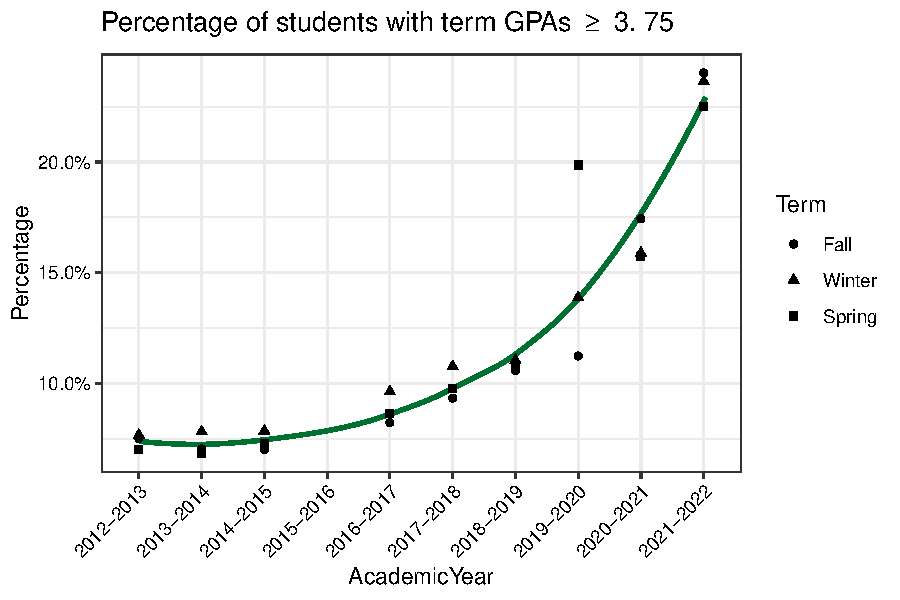
\includegraphics[width=\linewidth]{../visualizations/grade-inflation}
	\caption[Grade Inflation]{Percentage of all UO students on the Dean's List, which is essentially the percentage of full time students with term GPAs of 3.75 or above. Trendline fitted with LOESS in R (a type of local polynomial regression fitting).}
	\label{fig:grade-inflation}
\end{figure}


\subsection{Discussion, Threats to Validity, and Takeaways}

\textbf{Takeaway 1}: The percentage of students on the Dean's List -- essentially full time undergraduate students with more than 3.75 term GPAs -- has increased from about 7\% in Spring 2012 to 23\% in Spring 2022.

\textbf{Discussion and Threats to Validity}: It could be tempting to look at this data and assert that grade inflation is the culprit. That is to say, professors/career instructors/graduate employees have become more lenient in their grading in the last few years. However, there are at least three points to consider which add complexity or outright rebuttal to this conclusion.

\begin{enumerate}
	\item There may be a bimodal or multimodal separation of the GPA distribution data happening over time. That is to say, while there are more students meeting the 3.75 term GPA threshold today than in the past, other students might be failing or barely passing at greater rates, too. Without looking at the entire distribution of student grades over time, it's impossible to determine whether all students are seeing grade increases, if the ``middle class'' / B-range students are slowly disappearing to two sets of ``A'' students and ``C/D/F'' students, or some other phenomena is occurring. Since this GPA data is likely protected under law by FERPA, only UO itself -- likely through the Office of the Provost -- would be able to answer this question fully.
	\item As UO's profile increases, we are attracting and admitting more prepared students. These students are then able to meet the bar for academic excellence, which then puts them on the Dean's List. Similarly, UO's initiatives for wrap-around student support means more students that would have previously been off the Dean's List are now on it.
	\item Student grade grubbing is way up. Dealing with grade grubbing students is an emotional toll on the instructor. My sister-in-law is an English adjunct at a university in Texas. She got yet another nasty email from a student dissatisfied with his final grade on Christmas morning this last year. It takes an emotional toll to deal with these kinds of students, and I'm sure for some faculty there's a mental cost-benefit calculation done about the hassle of giving a lower grade for some students, especially if they feel unsupported and underpaid by the university.
\end{enumerate}

So what are the drivers of this trend of more students making the Dean's List? Hard to definitively say. But some combination of the above three points is likely.

Moreover, it's important to note that the trend started before COVID hit. Fall 2019, with 11\% of enrolled students on the Dean's List, was certainly higher than Fall 2012 at 8\%. It's clear that the COVID years accelerated the trend, however. It will be interesting to see how Fall 2022 data compare.

Future work around this research question revolves around whether other universities have seen similar grade distribution changes as UO. While it may be tempting for some members of the university community to assign lower grades to combat perceived grade inflation, doing so will only put UO's students at a competitive disadvantage when they seek out employment or external scholarships if UO student grades are consistently lower than their peers from otherwise similar universities. Understanding how UO's grade distribution compares to peers is important to determine before policymakers (whether individual instructors or academic leadership) make changes.

\section{RQ2: Are high performing students more likely to be Men or Women at UO?}

\subsection{Methodology}

In addition to the \textit{Around the O} articles about the Dean's List discussed in \S\ref{sec:rq1-methodology}, the actual Dean's List itself is a searchable Microsoft Excel spreadsheet. All lists are published in \textit{Around the O} or its archives from academic year 2012-2013 to 2021-2022, except for academic year 2015-2016 and Spring Term 2013. The list contains a student's first name, middle name, last name, major, home state, city, and zipcode. A student's gender is not included in the data.

To infer a student's gender, we employ \texttt{genderComputer}\footnote{\url{https://github.com/tue-mdse/genderComputer}}, a tool used in previous peer reviewed research for inferring gender from names. Provided a name, it infers ``Male,'' ``Female,'' ``Unisex,'' or ``Unknown.'' The tool has a reported precision of 93\%. We combine unisex and unknown into the same category for reporting purposes.

%We infer a student's gender by deploying the tool on a student's first name. If the tool is unable to determine Male or Female from a student's first name alone, we then apply the tool to the student's middle name (if any) to infer gender.


This gender inferment from the Dean's Lists is benchmarked against university-wide undergraduate gender enrollment ratios published at \url{https://provost.uoregon.edu/analytics/dashboards}, which is available only for Fall terms.

\subsection{Results}

% Please add the following required packages to your document preamble:
% \usepackage{longtable}
% Note: It may be necessary to compile the document several times to get a multi-page table to line up properly
\begin{longtable}[c]{|l|l|l|l|l|}
	\caption{\parbox{0.7\linewidth}{Gender distribution as a percentage of the Dean's List (i.e., had term GPAs of 3.75 or above) for each term with data. Missing entries indicate that the Dean's List was not available for that particular term. Rows may not sum to 100 due to rounding. }}
	\label{tab:gender-tab1}\\
	\hline
	\textbf{Academic Year} & \textbf{Term} & \textbf{Men} & \textbf{Women} & \textbf{Unknown} \\ \hline
	\endhead
	%
	2012-2013              & Fall          & 36\%           & 56\%             & 8\%              \\ \hline
	2012-2013              & Winter        & 37\%           & 54\%             & 9\%              \\ \hline
	2012-2013              & Spring        &                &                  &                  \\ \hline
	2013-2014              & Fall          & 39\%           & 54\%             & 7\%              \\ \hline
	2013-2014              & Winter        & 38\%           & 55\%             & 7\%              \\ \hline
	2013-2014              & Spring        & 37\%           & 55\%             & 7\%              \\ \hline
	2014-2015              & Fall          & 37\%           & 55\%             & 7\%              \\ \hline
	2014-2015              & Winter        & 38\%           & 54\%             & 8\%              \\ \hline
	2014-2015              & Spring        & 36\%           & 55\%             & 9\%              \\ \hline
	2015-2016              & Fall          &                &                  &                  \\ \hline
	2015-2016              & Winter        &                &                  &                  \\ \hline
	2015-2016              & Spring        &                &                  &                  \\ \hline
	2016-2017              & Fall          & 34\%           & 57\%             & 9\%              \\ \hline
	2016-2017              & Winter        & 33\%           & 58\%             & 9\%              \\ \hline
	2016-2017              & Spring        & 34\%           & 58\%             & 8\%              \\ \hline
	2017-2018              & Fall          & 35\%           & 58\%             & 7\%              \\ \hline
	2017-2018              & Winter        & 34\%           & 58\%             & 8\%              \\ \hline
	2017-2018              & Spring        & 34\%           & 58\%             & 8\%              \\ \hline
	2018-2019              & Fall          & 35\%           & 58\%             & 7\%              \\ \hline
	2018-2019              & Winter        & 36\%           & 57\%             & 7\%              \\ \hline
	2018-2019              & Spring        & 35\%           & 57\%             & 8\%              \\ \hline
	2019-2020              & Fall          & 36\%           & 57\%             & 7\%              \\ \hline
	2019-2020              & Winter        & 38\%           & 55\%             & 7\%              \\ \hline
	2019-2020              & Spring        & 37\%           & 55\%             & 8\%              \\ \hline
	2020-2021              & Fall          & 35\%           & 58\%             & 7\%              \\ \hline
	2020-2021              & Winter        & 35\%           & 57\%             & 8\%              \\ \hline
	2020-2021              & Spring        & 35\%           & 57\%             & 7\%              \\ \hline
	2021-2022              & Fall          & 38\%           & 55\%             & 7\%              \\ \hline
	2021-2022              & Winter        & 38\%           & 55\%             & 7\%              \\ \hline
	2021-2022              & Spring        & 38\%           & 55\%             & 7\%              \\ \hline
\end{longtable}

% Please add the following required packages to your document preamble:
% \usepackage{multirow}
% \usepackage{longtable}
% Note: It may be necessary to compile the document several times to get a multi-page table to line up properly
\begin{longtable}[c]{|l|l|ll|ll|l|}
	\caption{Two-gender ratio of Dean's List students (i.e., gender ratio with ``Unknowns'' excluded) compared with undergraduate enrollment by gender for the Fall enrollment census. Gender parity on the Dean's List would mean that the gender ratios of the Dean's List matched the gender ratios of overall enrollment.  Missing entries indicate that the Dean's List was not available for that particular term.}
	\label{tab:gender-benchmark}\\
	\hline
	\multicolumn{1}{|c|}{\multirow{2}{*}{\textbf{Academic Year}}} & \multicolumn{1}{c|}{\multirow{2}{*}{\textbf{Term}}} & \multicolumn{2}{c|}{\textbf{Men's Ratios}}                                           & \multicolumn{2}{c|}{\textbf{Women's Ratios}}                                         & \multicolumn{1}{c|}{\multirow{2}{*}{\parbox{1.75in}{\textbf{Women's Overrepresentation on Dean's List}}}} \\ \cline{3-6}
	\multicolumn{1}{|c|}{}                                        & \multicolumn{1}{c|}{}                               & \multicolumn{1}{c|}{\textit{Dean's List}} & \multicolumn{1}{c|}{\textit{Enrollment}} & \multicolumn{1}{c|}{\textit{Dean's List}} & \multicolumn{1}{c|}{\textit{Enrollment}} & \multicolumn{1}{c|}{}                                                                    \\ \hline
	\endhead
	%
	2012-2013                                                     & Fall                                                & \multicolumn{1}{l|}{39\%}                 & 46\%                                     & \multicolumn{1}{l|}{61\%}                 & 54\%                                     & 7\%                                                                                      \\ \hline
	2013-2014                                                     & Fall                                                & \multicolumn{1}{l|}{42\%}                 & 46\%                                     & \multicolumn{1}{l|}{58\%}                 & 54\%                                     & 4\%                                                                                      \\ \hline
	2014-2015                                                     & Fall                                                & \multicolumn{1}{l|}{40\%}                 & 46\%                                     & \multicolumn{1}{l|}{60\%}                 & 54\%                                     & 6\%                                                                                      \\ \hline
	2015-2016                                                     & Fall                                                & \multicolumn{1}{l|}{}                     & 44\%                                     & \multicolumn{1}{l|}{}                     & 56\%                                     &                                                                                          \\ \hline
	2016-2017                                                     & Fall                                                & \multicolumn{1}{l|}{37\%}                 & 45\%                                     & \multicolumn{1}{l|}{63\%}                 & 55\%                                     & 8\%                                                                                      \\ \hline
	2017-2018                                                     & Fall                                                & \multicolumn{1}{l|}{38\%}                 & 46\%                                     & \multicolumn{1}{l|}{62\%}                 & 54\%                                     & 8\%                                                                                      \\ \hline
	2018-2019                                                     & Fall                                                & \multicolumn{1}{l|}{38\%}                 & 46\%                                     & \multicolumn{1}{l|}{62\%}                 & 54\%                                     & 8\%                                                                                      \\ \hline
	2019-2020                                                     & Fall                                                & \multicolumn{1}{l|}{39\%}                 & 44\%                                     & \multicolumn{1}{l|}{61\%}                 & 56\%                                     & 5\%                                                                                      \\ \hline
	2020-2021                                                     & Fall                                                & \multicolumn{1}{l|}{38\%}                 & 43\%                                     & \multicolumn{1}{l|}{62\%}                 & 57\%                                     & 5\%                                                                                      \\ \hline
	2021-2022                                                     & Fall                                                & \multicolumn{1}{l|}{41\%}                 & 43\%                                     & \multicolumn{1}{l|}{59\%}                 & 57\%                                     & 2\%                                                                                      \\ \hline
\end{longtable}

\begin{figure}[H]
	\centering
	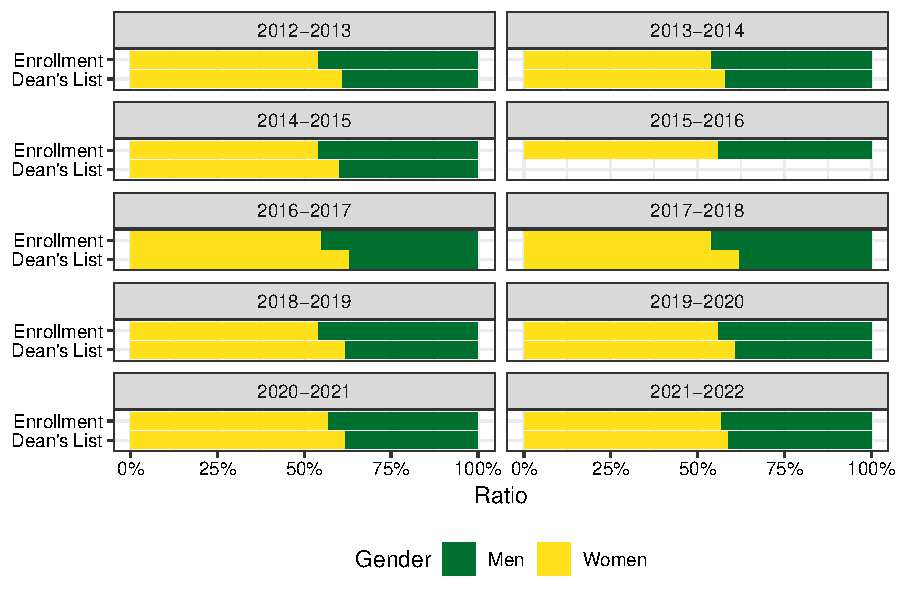
\includegraphics[width=\linewidth]{../visualizations/gender3}
	\caption[Gender differences]{Visualization of men vs women ratios on the Dean's List, compared with enrollment ratios for each Fall of the past 10 academic years. Women are consistently a greater percentage of students than men on the Dean's List, even when considering their greater enrollment numbers. The Dean's List for academic year 2015-2016 was not available online, which is why it's missing.}
	\label{fig:gender}
\end{figure}


\subsection{Discussion, Threats to Validity, and Takeaways}

\textbf{Takeaway 2}: Our results indicate that, for the last decade, women at UO are more likely than men to be on the Dean's List. If one believes the Dean's List to be an accurate set of UO's top students, then these findings suggest women are more likely than men to be among the top academic performers at UO. On average, women are overrepresented among top performing students by an additional 6\%, even when considering overall enrollment ratios. That is, 6\% is the average of the ``Women's Overrepresentation on Dean's List'' column in Table~\ref{tab:gender-benchmark}).

\textbf{Discussion and Threats to Validity}:

There are at least two threats to the validity of these results.

\begin{enumerate}
	\item The gender of each student is essentially an educated guess, not a self-report. To rectify this issue, the university would have to provide the self-identified gender data for each student on the various Dean's Lists. This is possibly a FERPA violation.
	\item Even with respect to UO's own published data, gender identities besides man and woman (or sex categories male and female) are not included. Understanding how non-binary gender identities fall on this distribution is important future work.
\end{enumerate}

Assuming that the true gender ratios of the Dean's List closely mirror the results presented here, however, leads to the question, ``\textit{Well, why are these results the way they are? Is there bias against men at UO?}'' Which is great future work for someone else to answer.

\section{RQ3: Which majors produce students with higher GPAs?}

\subsection{Methodology}

The ideal thing to do is get a list of enrollment by major for each term for the last decade and compare it with the number of students in each major on the Dean's List.

Unfortunately, I cannot find such a list of enrollment by major by term for the last decade. What I can find are some data dashboards from the Office of the Provost\footnote{\url{https://provost.uoregon.edu/analytics/dashboards}}, Institutional Research\footnote{\url{https://ir.uoregon.edu/students}}, and Registrar's Office\footnote{\url{https://registrar.uoregon.edu/statistics/majors}}. Neither of these websites have university wide major-specific data. But there is university-wide department-specific data. This is a subtle but important difference. As an illustrative example, the Department of Computer Science offers several majors: Computer Science, MACS (a Math + CS combo major), an accelerated BS+MS major, and so forth.

Moreover, one has to manually select the department to get the headcount. There's no way to just download the data as a spreadsheet, and I'm not manually collecting 30 terms $\times$ dozens of departments worth of enrollment data from obnoxious dropdown menus. It's winter break; I want to drink eggnog and play board games with my family, not waste time scraping data for this side project.

So instead, we're (1) aggregating the majors in the Dean's Lists to determine the most common majors on the Dean's List, (2) seeing if there's a nice curve to the distribution of the data to determine if there's an obvious elbow, and (3) comparing those frequently seen majors on the Dean's List against departmental enrollment data.

The goal is to find outliers amongst the top-producing departments relative to their undergraduate enrollments. For example, we hypothesize that Psychology -- long one of the most popular undergraduate majors, if not \textit{the} most popular major -- will show up in the list of most frequent majors on the Dean's List. But, we want to control for student headcount, so we'll divide by the Psychology department's enrollment to get its overall Dean's List production rate.

The result will be a short list where we can identify departments which (i) produce lots of Dean's List students and (ii) produce them at a rate greater than would be expected given the size of their department.

Further, to help benchmark, we'll (4) consider the \textit{Dean's List / Departmental Enrollment} ratio of the median majors by overall Dean's List prevalence to help establish a baseline ``typical'' Dean's List production rate.

Lastly, we will also (5) list all majors by Dean's List production year-over-year and identify increases/decreases.

\subsection{Results}
Our methodology had five steps: (1) aggregate the majors in the Dean's Lists to determine the most common majors on the Dean's List, (2) see if there's a nice curve to the distribution of the data to determine if there's an obvious elbow, (3) compare those frequently seen majors on the Dean's List against departmental enrollment data, (4) consider the \textit{Dean's List / Departmental Enrollment} ratio of the median majors by overall Dean's List prevalence to help establish a baseline ``typical'' Dean's List production rate, and (5) compare year-over-year figures.

We take each of these in turn.

\subsubsection{Steps 1 and 2: Major aggregation and distribution analysis}

\qquad

\begin{figure}[H]
	\centering
	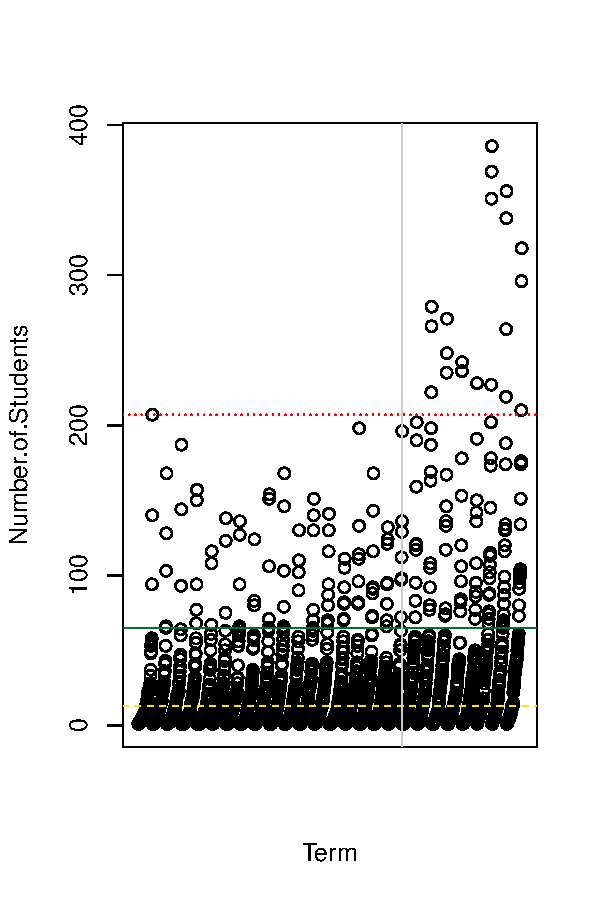
\includegraphics[width=0.33\linewidth]{../visualizations/contributions-by-major2}
	\caption{Each dot represents the number of students each major contributes to the Dean's List. Each roughly vertical line of dots represents an academic term in the last decade (four terms are missing due to missing data in academic year 2015-2016 and Spring 2013. The solid green horizontal line, which was arbitrarily placed, represents the 90th percentile or 65 students. This is to say that, across the last decade, 90\% of all majors contribute fewer than 65 students to the Dean's List each term. 10\% of majors contribute more than 65 students. The dashed yellow line is the median value, 13 students. While not in the methodology, we include a vertical gray line to denote the start of COVID (Winter 2020), and a red dotted line to indicate the most number of students a major ever produced on the Dean's List before COVID. }
	\label{fig:contributions-by-major}
\end{figure}


\subsubsection{Steps 3: List of most frequently seen majors against enrollment data}

There are 206 major-term points that have produced more than 65 students  on the Dean's List since 2012. These are the points above the green line in Figure~\ref{fig:contributions-by-major}.

%I found it interesting to separate the consolidated majors by a ``COVID'' line in Winter 2020.

\textbf{Majors which produced more than 65 students on the Dean's List at least once before Winter 2020}:

\begin{itemize}
\item Accounting
\item Biology
\item Pre-Business Administration
\item Business Administration
\item Economics
\item Educational Foundations
\item Exploring / Undeclared
\item General Social Science
\item Human Physiology
\item Jour:Advertising
\item Jour:Public Relations
\item Journalism
\item Political Science
\item Psychology
\end{itemize}


\textbf{Majors which produced more than 65 students on the Dean's List at least once after or during Winter 2020} (Bolded majors are not on the Pre-COVID list.):

\begin{itemize}
\item \textbf{Art}
\item Biology
\item Pre-Business Administration
\item Business Administration
\item \textbf{Cinema Studies}
\item \textbf{Communication Disorders and Sci}
\item \textbf{Computer and Information Science}
\item Economics
\item Educational Foundations
\item \textbf{English}
\item \textbf{Environmental Science}
\item \textbf{Environmental Studies}
\item Exploring / Undeclared
\item \textbf{Family and Human Services}
\item General Social Science
\item Human Physiology
\item Jour:Advertising
\item Jour:Public Relations
\item Journalism
\item Political Science
\item Psychology
\item \textbf{Sociology}
\end{itemize}

There are 20 majors-term points since COVID hit that have produced more Dean's List students than before COVID (which was 207 students in Fall 2012, majoring in ``Undeclared/Exploring''). These are the points above the red dotted line in Figure~\ref{fig:contributions-by-major}. While all major-term points above the green line are suspect, the ones above the red are particularly noteworthy. Of those major-term points above the red line, there were only five majors:

\begin{itemize}
	\item Pre-Business Administration
	\item Business Administration
	\item Psychology
	\item Political Science
	\item Undeclared / Exploring
\end{itemize}

%All of these majors were in the top producing majors pre-COVID, too.

%(Pre) Business Administration, Psychology, and Political Science are all incredibly popular majors, so sharp increases in student achievement on the Dean's List don't immediately strike me as out of line with other departments.

Why haven't I pulled together the department data? I'm feeling lazy (and I promised in the abstract that this is a half-assed report), so I'm not finishing Step 3 or 4 and pulling down the data to cross compare against department enrollments. Feel free to do that yourself: \url{https://provost.uoregon.edu/analytics/dashboards}

I did investigate almost all of the bolded majors in the list of post-COVID producers. In almost every case, total enrollment in these majors was either flat over the last decade or on the decline.



\subsubsection{Steps 5: Compare year-over-year figures}

\qquad


% Please add the following required packages to your document preamble:
% \usepackage{multirow}
% \usepackage{longtable}
% Note: It may be necessary to compile the document several times to get a multi-page table to line up properly

\small
\begin{longtable}[c]{|ccccc|}
	\caption{Pre-COVID and COVID Era comparison. The table is partitioned by majors which, on median, contributed more than 10 students to the Dean's List and those which contributed less.  In the first section, rows are sorted by percentage of change. In the second section of majors which contributed 10 or fewer students, the rows are sorted by the numerical change.}
	\label{tab:pre-post-covid}\\
	\hline
	\multicolumn{1}{|c|}{\multirow{2}{*}{\textbf{Major}}}            & \multicolumn{2}{c|}{\textbf{Students on Dean's List (Medians)}}                                                 & \multicolumn{2}{c|}{\textbf{Change Since Covid Hit}} \\ \cline{2-5} 
	\multicolumn{1}{|c|}{}                                           & \multicolumn{1}{c|}{\textbf{F2016 to F2019}} & \multicolumn{1}{c|}{\textbf{W2020 to S2021}} & \multicolumn{1}{c|}{\textbf{Number}}    & \textbf{Percentage}   \\ \hline
	\endhead
	%
	\multicolumn{5}{|c|}{\textbf{Majors with more than 10 students (median) on the Dean's List from Fall 2016 to Fall 2019}}                                                                                                                             \\ \hline
	\multicolumn{1}{|c|}{Business Administration}                    & \multicolumn{1}{c|}{70}                              & \multicolumn{1}{c|}{275}                                 & \multicolumn{1}{c|}{205}                & 293\%                 \\ \hline
	\multicolumn{1}{|c|}{Family and Human Services}                  & \multicolumn{1}{c|}{14}                              & \multicolumn{1}{c|}{52}                                  & \multicolumn{1}{c|}{38}                 & 271\%                 \\ \hline
	\multicolumn{1}{|c|}{Product Design}                             & \multicolumn{1}{c|}{13}                              & \multicolumn{1}{c|}{40}                                  & \multicolumn{1}{c|}{27}                 & 208\%                 \\ \hline
	\multicolumn{1}{|c|}{Jour:Advertising}                           & \multicolumn{1}{c|}{60}                              & \multicolumn{1}{c|}{160}                                 & \multicolumn{1}{c|}{100}                & 167\%                 \\ \hline
	\multicolumn{1}{|c|}{Music Performance}                          & \multicolumn{1}{c|}{11}                              & \multicolumn{1}{c|}{29}                                  & \multicolumn{1}{c|}{18}                 & 164\%                 \\ \hline
	\multicolumn{1}{|c|}{Cinema Studies}                             & \multicolumn{1}{c|}{23}                              & \multicolumn{1}{c|}{58}                                  & \multicolumn{1}{c|}{35}                 & 152\%                 \\ \hline
	\multicolumn{1}{|c|}{Jour:Public Relations}                      & \multicolumn{1}{c|}{39}                              & \multicolumn{1}{c|}{98}                                  & \multicolumn{1}{c|}{59}                 & 151\%                 \\ \hline
	\multicolumn{1}{|c|}{Journalism}                                 & \multicolumn{1}{c|}{38}                              & \multicolumn{1}{c|}{91}                                  & \multicolumn{1}{c|}{53}                 & 139\%                 \\ \hline
	\multicolumn{1}{|c|}{Psychology}                                 & \multicolumn{1}{c|}{119}                             & \multicolumn{1}{c|}{257}                                 & \multicolumn{1}{c|}{138}                & 116\%                 \\ \hline
	\multicolumn{1}{|c|}{Chemistry}                                  & \multicolumn{1}{c|}{12}                              & \multicolumn{1}{c|}{26}                                  & \multicolumn{1}{c|}{14}                 & 117\%                 \\ \hline
	\multicolumn{1}{|c|}{Music Education}                            & \multicolumn{1}{c|}{11}                              & \multicolumn{1}{c|}{23}                                  & \multicolumn{1}{c|}{12}                 & 109\%                 \\ \hline
	\multicolumn{1}{|c|}{Political Science}                          & \multicolumn{1}{c|}{81}                              & \multicolumn{1}{c|}{165}                                 & \multicolumn{1}{c|}{84}                 & 104\%                 \\ \hline
	\multicolumn{1}{|c|}{Art}                                        & \multicolumn{1}{c|}{29}                              & \multicolumn{1}{c|}{56}                                  & \multicolumn{1}{c|}{27}                 & 93\%                  \\ \hline
	\multicolumn{1}{|c|}{Educational Foundations}                    & \multicolumn{1}{c|}{43}                              & \multicolumn{1}{c|}{81}                                  & \multicolumn{1}{c|}{38}                 & 88\%                  \\ \hline
	\multicolumn{1}{|c|}{Physics}                                    & \multicolumn{1}{c|}{14}                              & \multicolumn{1}{c|}{27}                                  & \multicolumn{1}{c|}{13}                 & 93\%                  \\ \hline
	\multicolumn{1}{|c|}{History}                                    & \multicolumn{1}{c|}{23}                              & \multicolumn{1}{c|}{42}                                  & \multicolumn{1}{c|}{19}                 & 83\%                  \\ \hline
	\multicolumn{1}{|c|}{Linguistics}                                & \multicolumn{1}{c|}{12}                              & \multicolumn{1}{c|}{22}                                  & \multicolumn{1}{c|}{10}                 & 83\%                  \\ \hline
	\multicolumn{1}{|c|}{Environmental Science}                      & \multicolumn{1}{c|}{23}                              & \multicolumn{1}{c|}{41}                                  & \multicolumn{1}{c|}{18}                 & 78\%                  \\ \hline
	\multicolumn{1}{|c|}{Biochemistry}                               & \multicolumn{1}{c|}{22}                              & \multicolumn{1}{c|}{39}                                  & \multicolumn{1}{c|}{17}                 & 77\%                  \\ \hline
	\multicolumn{1}{|c|}{Environmental Studies}                      & \multicolumn{1}{c|}{33}                              & \multicolumn{1}{c|}{58}                                  & \multicolumn{1}{c|}{25}                 & 76\%                  \\ \hline
	\multicolumn{1}{|c|}{Human Physiology}                           & \multicolumn{1}{c|}{89}                              & \multicolumn{1}{c|}{149}                                 & \multicolumn{1}{c|}{60}                 & 67\%                  \\ \hline
	\multicolumn{1}{|c|}{General Social Science}                     & \multicolumn{1}{c|}{31}                              & \multicolumn{1}{c|}{52}                                  & \multicolumn{1}{c|}{21}                 & 68\%                  \\ \hline
	\multicolumn{1}{|c|}{Architecture}                               & \multicolumn{1}{c|}{23}                              & \multicolumn{1}{c|}{39}                                  & \multicolumn{1}{c|}{16}                 & 70\%                  \\ \hline
	\multicolumn{1}{|c|}{Art and Technology}                         & \multicolumn{1}{c|}{21}                              & \multicolumn{1}{c|}{35}                                  & \multicolumn{1}{c|}{14}                 & 67\%                  \\ \hline
	\multicolumn{1}{|c|}{Anthropology}                               & \multicolumn{1}{c|}{18}                              & \multicolumn{1}{c|}{30}                                  & \multicolumn{1}{c|}{12}                 & 67\%                  \\ \hline
	\multicolumn{1}{|c|}{Communication Disorders \& Sci}             & \multicolumn{1}{c|}{30}                              & \multicolumn{1}{c|}{47}                                  & \multicolumn{1}{c|}{17}                 & 57\%                  \\ \hline
	\multicolumn{1}{|c|}{Sociology}                                  & \multicolumn{1}{c|}{32}                              & \multicolumn{1}{c|}{49}                                  & \multicolumn{1}{c|}{17}                 & 53\%                  \\ \hline
	\multicolumn{1}{|c|}{Biology}                                    & \multicolumn{1}{c|}{68}                              & \multicolumn{1}{c|}{105}                                 & \multicolumn{1}{c|}{37}                 & 54\%                  \\ \hline
	\multicolumn{1}{|c|}{Computer \& Information Science}            & \multicolumn{1}{c|}{38}                              & \multicolumn{1}{c|}{58}                                  & \multicolumn{1}{c|}{20}                 & 53\%                  \\ \hline
	\multicolumn{1}{|c|}{Accounting}                                 & \multicolumn{1}{c|}{27}                              & \multicolumn{1}{c|}{42}                                  & \multicolumn{1}{c|}{15}                 & 56\%                  \\ \hline
	\multicolumn{1}{|c|}{General Science}                            & \multicolumn{1}{c|}{12}                              & \multicolumn{1}{c|}{17}                                  & \multicolumn{1}{c|}{5}                  & 42\%                  \\ \hline
	\multicolumn{1}{|c|}{Philosophy}                                 & \multicolumn{1}{c|}{11}                              & \multicolumn{1}{c|}{15}                                  & \multicolumn{1}{c|}{4}                  & 36\%                  \\ \hline
	\multicolumn{1}{|c|}{Economics}                                  & \multicolumn{1}{c|}{42}                              & \multicolumn{1}{c|}{54}                                  & \multicolumn{1}{c|}{12}                 & 29\%                  \\ \hline
	\multicolumn{1}{|c|}{Exploring / Undeclared}                     & \multicolumn{1}{c|}{149}                             & \multicolumn{1}{c|}{189}                                 & \multicolumn{1}{c|}{40}                 & 27\%                  \\ \hline
	\multicolumn{1}{|c|}{Mathematics}                                & \multicolumn{1}{c|}{22}                              & \multicolumn{1}{c|}{26}                                  & \multicolumn{1}{c|}{4}                  & 18\%                  \\ \hline
	\multicolumn{1}{|c|}{Spanish}                                    & \multicolumn{1}{c|}{14}                              & \multicolumn{1}{c|}{15}                                  & \multicolumn{1}{c|}{1}                  & 7\%                   \\ \hline
	\multicolumn{1}{|c|}{English}                                    & \multicolumn{1}{c|}{54}                              & \multicolumn{1}{c|}{57}                                  & \multicolumn{1}{c|}{3}                  & 6\%                   \\ \hline
	\multicolumn{1}{|c|}{Pre-Journalism}                             & \multicolumn{1}{c|}{51}                              & \multicolumn{1}{c|}{52}                                  & \multicolumn{1}{c|}{1}                  & 2\%                   \\ \hline
	\multicolumn{1}{|c|}{Pre-Business Administration}                & \multicolumn{1}{c|}{122}                             & \multicolumn{1}{c|}{119}                                 & \multicolumn{1}{c|}{-3}                 & -2\%                  \\ \hline
	\multicolumn{1}{|c|}{Theater Arts}                               & \multicolumn{1}{c|}{14}                              & \multicolumn{1}{c|}{14}                                  & \multicolumn{1}{c|}{0}                  & 0\%                   \\ \hline
	\multicolumn{1}{|c|}{Music}                                      & \multicolumn{1}{c|}{36}                              & \multicolumn{1}{c|}{31}                                  & \multicolumn{1}{c|}{-5}                 & -14\%                 \\ \hline
	\multicolumn{1}{|c|}{International Studies}                      & \multicolumn{1}{c|}{20}                              & \multicolumn{1}{c|}{17}                                  & \multicolumn{1}{c|}{-3}                 & -15\%                 \\ \hline
	\multicolumn{1}{|c|}{Pre-International Studies}                  & \multicolumn{1}{c|}{29}                              & \multicolumn{1}{c|}{8}                                   & \multicolumn{1}{c|}{-21}                & -72\%                 \\ \hline
	\multicolumn{1}{|c|}{Pre-Education}                              & \multicolumn{1}{c|}{27}                              & \multicolumn{1}{c|}{0}                                   & \multicolumn{1}{c|}{-27}                & -100\%                \\ \hline
	\multicolumn{1}{|c|}{Pre-Family and Human Services}              & \multicolumn{1}{c|}{15}                              & \multicolumn{1}{c|}{0}                                   & \multicolumn{1}{c|}{-15}                & -100\%                \\ \hline
	\multicolumn{5}{|c|}{\textbf{Majors with 10 or fewer students (median) on the Dean's List from Fall 2016 to Fall 2019}}                                                                                                                              \\ \hline
	\multicolumn{1}{|c|}{Pre-Global Studies}                         & \multicolumn{1}{c|}{0}                               & \multicolumn{1}{c|}{23}                                  & \multicolumn{1}{c|}{23}                 & NA                    \\ \hline
	\multicolumn{1}{|c|}{Marine Biology}                             & \multicolumn{1}{c|}{10}                              & \multicolumn{1}{c|}{26}                                  & \multicolumn{1}{c|}{16}                 & 160\%                 \\ \hline
	\multicolumn{1}{|c|}{Pre-J:Advertising}                          & \multicolumn{1}{c|}{8}                               & \multicolumn{1}{c|}{22}                                  & \multicolumn{1}{c|}{14}                 & 175\%                 \\ \hline
	\multicolumn{1}{|c|}{Global Studies}                             & \multicolumn{1}{c|}{0}                               & \multicolumn{1}{c|}{12}                                  & \multicolumn{1}{c|}{12}                 & NA                    \\ \hline
	\multicolumn{1}{|c|}{Neuroscience}                               & \multicolumn{1}{c|}{0}                               & \multicolumn{1}{c|}{12}                                  & \multicolumn{1}{c|}{12}                 & NA                    \\ \hline
	\multicolumn{1}{|c|}{Pre-Planning Public Policy Mgm}             & \multicolumn{1}{c|}{8}                               & \multicolumn{1}{c|}{19}                                  & \multicolumn{1}{c|}{11}                 & 138\%                 \\ \hline
	\multicolumn{1}{|c|}{Pre-J:Public Relations}                     & \multicolumn{1}{c|}{3}                               & \multicolumn{1}{c|}{14}                                  & \multicolumn{1}{c|}{11}                 & 367\%                 \\ \hline
	\multicolumn{1}{|c|}{Planning Public Policy \& Mgmt}             & \multicolumn{1}{c|}{8}                               & \multicolumn{1}{c|}{17}                                  & \multicolumn{1}{c|}{9}                  & 113\%                 \\ \hline
	\multicolumn{1}{|c|}{Earth Sciences}                             & \multicolumn{1}{c|}{3}                               & \multicolumn{1}{c|}{9}                                   & \multicolumn{1}{c|}{6}                  & 200\%                 \\ \hline
	\multicolumn{1}{|c|}{Women's Gendr \& Sexuality St}              & \multicolumn{1}{c|}{1}                               & \multicolumn{1}{c|}{7}                                   & \multicolumn{1}{c|}{6}                  & 600\%                 \\ \hline
	\multicolumn{1}{|c|}{Mathematics \& Computer Science}            & \multicolumn{1}{c|}{4}                               & \multicolumn{1}{c|}{10}                                  & \multicolumn{1}{c|}{6}                  & 150\%                 \\ \hline
	\multicolumn{1}{|c|}{Pre-J:Media Studies}                        & \multicolumn{1}{c|}{1}                               & \multicolumn{1}{c|}{7}                                   & \multicolumn{1}{c|}{6}                  & 600\%                 \\ \hline
	\multicolumn{1}{|c|}{Data Science}                               & \multicolumn{1}{c|}{0}                               & \multicolumn{1}{c|}{6}                                   & \multicolumn{1}{c|}{6}                  & NA                    \\ \hline
	\multicolumn{1}{|c|}{Dance}                                      & \multicolumn{1}{c|}{4}                               & \multicolumn{1}{c|}{9}                                   & \multicolumn{1}{c|}{5}                  & 125\%                 \\ \hline
	\multicolumn{1}{|c|}{Geography}                                  & \multicolumn{1}{c|}{7}                               & \multicolumn{1}{c|}{11}                                  & \multicolumn{1}{c|}{4}                  & 57\%                  \\ \hline
	\multicolumn{1}{|c|}{Spatial Data Sci \& Technology}             & \multicolumn{1}{c|}{2}                               & \multicolumn{1}{c|}{6}                                   & \multicolumn{1}{c|}{4}                  & 200\%                 \\ \hline
	\multicolumn{1}{|c|}{Ethnic Studies}                             & \multicolumn{1}{c|}{4}                               & \multicolumn{1}{c|}{8}                                   & \multicolumn{1}{c|}{4}                  & 100\%                 \\ \hline
	\multicolumn{1}{|c|}{Art History}                                & \multicolumn{1}{c|}{3}                               & \multicolumn{1}{c|}{6}                                   & \multicolumn{1}{c|}{3}                  & 100\%                 \\ \hline
	\multicolumn{1}{|c|}{Chinese}                                    & \multicolumn{1}{c|}{3}                               & \multicolumn{1}{c|}{6}                                   & \multicolumn{1}{c|}{3}                  & 100\%                 \\ \hline
	\multicolumn{1}{|c|}{Pre-Landscape Architecture}                 & \multicolumn{1}{c|}{0}                               & \multicolumn{1}{c|}{3}                                   & \multicolumn{1}{c|}{3}                  & NA                    \\ \hline
	\multicolumn{1}{|c|}{Asian Studies}                              & \multicolumn{1}{c|}{3}                               & \multicolumn{1}{c|}{5}                                   & \multicolumn{1}{c|}{2}                  & 67\%                  \\ \hline
	\multicolumn{1}{|c|}{Comparative Literature}                     & \multicolumn{1}{c|}{5}                               & \multicolumn{1}{c|}{6}                                   & \multicolumn{1}{c|}{1}                  & 20\%                  \\ \hline
	\multicolumn{1}{|c|}{Classics}                                   & \multicolumn{1}{c|}{2}                               & \multicolumn{1}{c|}{4}                                   & \multicolumn{1}{c|}{2}                  & 100\%                 \\ \hline
	\multicolumn{1}{|c|}{Music Composition}                          & \multicolumn{1}{c|}{2}                               & \multicolumn{1}{c|}{3}                                   & \multicolumn{1}{c|}{1}                  & 50\%                  \\ \hline
	\multicolumn{1}{|c|}{Humanities}                                 & \multicolumn{1}{c|}{3}                               & \multicolumn{1}{c|}{4}                                   & \multicolumn{1}{c|}{1}                  & 33\%                  \\ \hline
	\multicolumn{1}{|c|}{Religious Studies}                          & \multicolumn{1}{c|}{1}                               & \multicolumn{1}{c|}{2}                                   & \multicolumn{1}{c|}{1}                  & 100\%                 \\ \hline
	\multicolumn{1}{|c|}{Folklore and Public Culture}                & \multicolumn{1}{c|}{0}                               & \multicolumn{1}{c|}{1}                                   & \multicolumn{1}{c|}{1}                  & NA                    \\ \hline
	\multicolumn{1}{|c|}{Italian}                                    & \multicolumn{1}{c|}{0}                               & \multicolumn{1}{c|}{1}                                   & \multicolumn{1}{c|}{1}                  & NA                    \\ \hline
	\multicolumn{1}{|c|}{Latin American Studies}                     & \multicolumn{1}{c|}{0}                               & \multicolumn{1}{c|}{1}                                   & \multicolumn{1}{c|}{1}                  & NA                    \\ \hline
	\multicolumn{1}{|c|}{French}                                     & \multicolumn{1}{c|}{2}                               & \multicolumn{1}{c|}{3}                                   & \multicolumn{1}{c|}{1}                  & 50\%                  \\ \hline
	\multicolumn{1}{|c|}{Landscape Architecture}                     & \multicolumn{1}{c|}{1}                               & \multicolumn{1}{c|}{1}                                   & \multicolumn{1}{c|}{0}                  & 0\%                   \\ \hline
	\multicolumn{1}{|c|}{Medieval Studies}                           & \multicolumn{1}{c|}{1}                               & \multicolumn{1}{c|}{1}                                   & \multicolumn{1}{c|}{0}                  & 0\%                   \\ \hline
	\multicolumn{1}{|c|}{Music: Jazz Studies}                        & \multicolumn{1}{c|}{7}                               & \multicolumn{1}{c|}{7}                                   & \multicolumn{1}{c|}{0}                  & 0\%                   \\ \hline
	\multicolumn{1}{|c|}{Jour:Media Studies}                         & \multicolumn{1}{c|}{6}                               & \multicolumn{1}{c|}{6}                                   & \multicolumn{1}{c|}{0}                  & 0\%                   \\ \hline
	\multicolumn{1}{|c|}{Arts Management}                            & \multicolumn{1}{c|}{0}                               & \multicolumn{1}{c|}{0}                                   & \multicolumn{1}{c|}{0}                  & 0\%                   \\ \hline
	\multicolumn{1}{|c|}{Ceramics}                                   & \multicolumn{1}{c|}{0}                               & \multicolumn{1}{c|}{0}                                   & \multicolumn{1}{c|}{0}                  & 0\%                   \\ \hline
	\multicolumn{1}{|c|}{Communication Disorders and Sciences}       & \multicolumn{1}{c|}{0}                               & \multicolumn{1}{c|}{0}                                   & \multicolumn{1}{c|}{0}                  & 0\%                   \\ \hline
	\multicolumn{1}{|c|}{Fibers}                                     & \multicolumn{1}{c|}{0}                               & \multicolumn{1}{c|}{0}                                   & \multicolumn{1}{c|}{0}                  & 0\%                   \\ \hline
	\multicolumn{1}{|c|}{Folklore}                                   & \multicolumn{1}{c|}{0}                               & \multicolumn{1}{c|}{0}                                   & \multicolumn{1}{c|}{0}                  & 0\%                   \\ \hline
	\multicolumn{1}{|c|}{Jour:Communication Studies}                 & \multicolumn{1}{c|}{0}                               & \multicolumn{1}{c|}{0}                                   & \multicolumn{1}{c|}{0}                  & 0\%                   \\ \hline
	\multicolumn{1}{|c|}{Journalism: Advertising}                    & \multicolumn{1}{c|}{0}                               & \multicolumn{1}{c|}{0}                                   & \multicolumn{1}{c|}{0}                  & 0\%                   \\ \hline
	\multicolumn{1}{|c|}{Journalism: Media Studies}                  & \multicolumn{1}{c|}{0}                               & \multicolumn{1}{c|}{0}                                   & \multicolumn{1}{c|}{0}                  & 0\%                   \\ \hline
	\multicolumn{1}{|c|}{Journalism: Public Relations}               & \multicolumn{1}{c|}{0}                               & \multicolumn{1}{c|}{0}                                   & \multicolumn{1}{c|}{0}                  & 0\%                   \\ \hline
	\multicolumn{1}{|c|}{Judaic Studies}                             & \multicolumn{1}{c|}{0}                               & \multicolumn{1}{c|}{0}                                   & \multicolumn{1}{c|}{0}                  & 0\%                   \\ \hline
	\multicolumn{1}{|c|}{Metalsmithing and Jewelry}                  & \multicolumn{1}{c|}{0}                               & \multicolumn{1}{c|}{0}                                   & \multicolumn{1}{c|}{0}                  & 0\%                   \\ \hline
	\multicolumn{1}{|c|}{Multidisciplinary Science}                  & \multicolumn{1}{c|}{0}                               & \multicolumn{1}{c|}{0}                                   & \multicolumn{1}{c|}{0}                  & 0\%                   \\ \hline
	\multicolumn{1}{|c|}{Music: Pre Teacher Licensure}               & \multicolumn{1}{c|}{0}                               & \multicolumn{1}{c|}{0}                                   & \multicolumn{1}{c|}{0}                  & 0\%                   \\ \hline
	\multicolumn{1}{|c|}{Painting}                                   & \multicolumn{1}{c|}{0}                               & \multicolumn{1}{c|}{0}                                   & \multicolumn{1}{c|}{0}                  & 0\%                   \\ \hline
	\multicolumn{1}{|c|}{Photography}                                & \multicolumn{1}{c|}{0}                               & \multicolumn{1}{c|}{0}                                   & \multicolumn{1}{c|}{0}                  & 0\%                   \\ \hline
	\multicolumn{1}{|c|}{Planning Public Policy \& Management}       & \multicolumn{1}{c|}{0}                               & \multicolumn{1}{c|}{0}                                   & \multicolumn{1}{c|}{0}                  & 0\%                   \\ \hline
	\multicolumn{1}{|c|}{Pre-J:Communication Studies}                & \multicolumn{1}{c|}{0}                               & \multicolumn{1}{c|}{0}                                   & \multicolumn{1}{c|}{0}                  & 0\%                   \\ \hline
	\multicolumn{1}{|c|}{Pre-Journalism: Advertising}                & \multicolumn{1}{c|}{0}                               & \multicolumn{1}{c|}{0}                                   & \multicolumn{1}{c|}{0}                  & 0\%                   \\ \hline
	\multicolumn{1}{|c|}{Pre-Journalism: Communication Studies}      & \multicolumn{1}{c|}{0}                               & \multicolumn{1}{c|}{0}                                   & \multicolumn{1}{c|}{0}                  & 0\%                   \\ \hline
	\multicolumn{1}{|c|}{Pre-Journalism: Public Relations}           & \multicolumn{1}{c|}{0}                               & \multicolumn{1}{c|}{0}                                   & \multicolumn{1}{c|}{0}                  & 0\%                   \\ \hline
	\multicolumn{1}{|c|}{Pre-Marine Biology}                         & \multicolumn{1}{c|}{0}                               & \multicolumn{1}{c|}{0}                                   & \multicolumn{1}{c|}{0}                  & 0\%                   \\ \hline
	\multicolumn{1}{|c|}{Pre-Planning Public Policy and Management}  & \multicolumn{1}{c|}{0}                               & \multicolumn{1}{c|}{0}                                   & \multicolumn{1}{c|}{0}                  & 0\%                   \\ \hline
	\multicolumn{1}{|c|}{Printmaking}                                & \multicolumn{1}{c|}{0}                               & \multicolumn{1}{c|}{0}                                   & \multicolumn{1}{c|}{0}                  & 0\%                   \\ \hline
	\multicolumn{1}{|c|}{Russ E Euro \& Eurasia Studies}             & \multicolumn{1}{c|}{0}                               & \multicolumn{1}{c|}{0}                                   & \multicolumn{1}{c|}{0}                  & 0\%                   \\ \hline
	\multicolumn{1}{|c|}{Russian \& East Europe Studies}             & \multicolumn{1}{c|}{0}                               & \multicolumn{1}{c|}{0}                                   & \multicolumn{1}{c|}{0}                  & 0\%                   \\ \hline
	\multicolumn{1}{|c|}{Russian East European and Eurasian Studies} & \multicolumn{1}{c|}{0}                               & \multicolumn{1}{c|}{0}                                   & \multicolumn{1}{c|}{0}                  & 0\%                   \\ \hline
	\multicolumn{1}{|c|}{Sculpture}                                  & \multicolumn{1}{c|}{0}                               & \multicolumn{1}{c|}{0}                                   & \multicolumn{1}{c|}{0}                  & 0\%                   \\ \hline
	\multicolumn{1}{|c|}{Unclassified/Continuing Educ}               & \multicolumn{1}{c|}{0}                               & \multicolumn{1}{c|}{0}                                   & \multicolumn{1}{c|}{0}                  & 0\%                   \\ \hline
	\multicolumn{1}{|c|}{Interior Architecture}                      & \multicolumn{1}{c|}{4}                               & \multicolumn{1}{c|}{3}                                   & \multicolumn{1}{c|}{-1}                 & -25\%                 \\ \hline
	\multicolumn{1}{|c|}{German}                                     & \multicolumn{1}{c|}{2}                               & \multicolumn{1}{c|}{2}                                   & \multicolumn{1}{c|}{0}                  & 0\%                   \\ \hline
	\multicolumn{1}{|c|}{Pre-Engineering}                            & \multicolumn{1}{c|}{1}                               & \multicolumn{1}{c|}{0}                                   & \multicolumn{1}{c|}{-1}                 & -100\%                \\ \hline
	\multicolumn{1}{|c|}{Romance Languages}                          & \multicolumn{1}{c|}{5}                               & \multicolumn{1}{c|}{4}                                   & \multicolumn{1}{c|}{-1}                 & -20\%                 \\ \hline
	\multicolumn{1}{|c|}{National Student Exchange}                  & \multicolumn{1}{c|}{1}                               & \multicolumn{1}{c|}{0}                                   & \multicolumn{1}{c|}{-1}                 & -100\%                \\ \hline
	\multicolumn{1}{|c|}{Japanese}                                   & \multicolumn{1}{c|}{8}                               & \multicolumn{1}{c|}{6}                                   & \multicolumn{1}{c|}{-2}                 & -25\%                 \\ \hline
	\multicolumn{1}{|c|}{Women's and Gender Studies}                 & \multicolumn{1}{c|}{2}                               & \multicolumn{1}{c|}{0}                                   & \multicolumn{1}{c|}{-2}                 & -100\%                \\ \hline
	\multicolumn{1}{|c|}{Geological Sciences}                        & \multicolumn{1}{c|}{3}                               & \multicolumn{1}{c|}{0}                                   & \multicolumn{1}{c|}{-3}                 & -100\%                \\ \hline
	\multicolumn{1}{|c|}{Digital Arts}                               & \multicolumn{1}{c|}{6}                               & \multicolumn{1}{c|}{0}                                   & \multicolumn{1}{c|}{-6}                 & -100\%                \\ \hline
	\multicolumn{1}{|c|}{Material \& Product Studies}                & \multicolumn{1}{c|}{9}                               & \multicolumn{1}{c|}{0}                                   & \multicolumn{1}{c|}{-9}                 & -100\%                \\ \hline
\end{longtable}

% Please add the following required packages to your document preamble:
% \usepackage{longtable}
% Note: It may be necessary to compile the document several times to get a multi-page table to line up properly
\begin{landscape}
\tiny
\begin{longtable}[c]{|ccccccccccccccccccc|}
	\caption{Term-over-Term comparison. The table is partitioned by majors which, on median, contributed more than 10 students to the Dean's List and those which contributed less.  In the first section, rows are sorted by percentage of change. In the second section of majors which contributed 10 or fewer students, the rows are sorted by the numerical change.}
	\label{tab:term-over-term-numbers}\\
	\hline
	\multicolumn{1}{|c|}{\textbf{Academic Year}}                     & \multicolumn{3}{c|}{\textbf{2016-2017}}                                                             & \multicolumn{3}{c|}{\textbf{2017-2018}}                                                             & \multicolumn{3}{c|}{\textbf{2018-2019}}                                                             & \multicolumn{3}{c|}{\textbf{2019-2020}}                                                             & \multicolumn{3}{c|}{\textbf{2020-2021}}                                                             & \multicolumn{3}{c|}{\textbf{2021-2022}}                                        \\ \hline
	\endhead
	%
	\multicolumn{1}{|c|}{\textbf{Term (F:Fall, W:Winter, S:Spring)}} & \multicolumn{1}{c|}{\textbf{F}} & \multicolumn{1}{c|}{\textbf{W}} & \multicolumn{1}{c|}{\textbf{S}} & \multicolumn{1}{c|}{\textbf{F}} & \multicolumn{1}{c|}{\textbf{W}} & \multicolumn{1}{c|}{\textbf{S}} & \multicolumn{1}{c|}{\textbf{F}} & \multicolumn{1}{c|}{\textbf{W}} & \multicolumn{1}{c|}{\textbf{S}} & \multicolumn{1}{c|}{\textbf{F}} & \multicolumn{1}{c|}{\textbf{W}} & \multicolumn{1}{c|}{\textbf{S}} & \multicolumn{1}{c|}{\textbf{F}} & \multicolumn{1}{c|}{\textbf{W}} & \multicolumn{1}{c|}{\textbf{S}} & \multicolumn{1}{c|}{\textbf{F}} & \multicolumn{1}{c|}{\textbf{W}} & \textbf{S} \\ \hline
	\multicolumn{1}{|c|}{\textbf{Major}}                             & \multicolumn{10}{c|}{\textbf{Pre-COVID}}                                                                                                                                                                                                                                                                                                          & \multicolumn{8}{c|}{\textbf{COVID Era}}                                                                                                                                                                                                                  \\ \hline
	\multicolumn{19}{|c|}{\textbf{Majors with more than 10 students (median) on the Dean's List from Fall 2016 to Fall 2019}}                                                                                                                                                                                                                                                                                                                                                                                                                                                                                                                                                       \\ \hline
	\multicolumn{1}{|c|}{Business Administration}                    & \multicolumn{1}{c|}{49}         & \multicolumn{1}{c|}{50}         & \multicolumn{1}{c|}{42}         & \multicolumn{1}{c|}{63}         & \multicolumn{1}{c|}{68}         & \multicolumn{1}{c|}{71}         & \multicolumn{1}{c|}{111}        & \multicolumn{1}{c|}{116}        & \multicolumn{1}{c|}{124}        & \multicolumn{1}{c|}{136}        & \multicolumn{1}{c|}{202}        & \multicolumn{1}{c|}{279}        & \multicolumn{1}{c|}{271}        & \multicolumn{1}{c|}{236}        & \multicolumn{1}{c|}{228}        & \multicolumn{1}{c|}{386}        & \multicolumn{1}{c|}{338}        & 296        \\ \hline
	\multicolumn{1}{|c|}{Family and Human Services}                  & \multicolumn{1}{c|}{13}         & \multicolumn{1}{c|}{13}         & \multicolumn{1}{c|}{9}          & \multicolumn{1}{c|}{15}         & \multicolumn{1}{c|}{16}         & \multicolumn{1}{c|}{11}         & \multicolumn{1}{c|}{18}         & \multicolumn{1}{c|}{22}         & \multicolumn{1}{c|}{8}          & \multicolumn{1}{c|}{20}         & \multicolumn{1}{c|}{38}         & \multicolumn{1}{c|}{60}         & \multicolumn{1}{c|}{57}         & \multicolumn{1}{c|}{40}         & \multicolumn{1}{c|}{46}         & \multicolumn{1}{c|}{57}         & \multicolumn{1}{c|}{68}         & 45         \\ \hline
	\multicolumn{1}{|c|}{Product Design}                             & \multicolumn{1}{c|}{5}          & \multicolumn{1}{c|}{7}          & \multicolumn{1}{c|}{4}          & \multicolumn{1}{c|}{8}          & \multicolumn{1}{c|}{15}         & \multicolumn{1}{c|}{10}         & \multicolumn{1}{c|}{34}         & \multicolumn{1}{c|}{28}         & \multicolumn{1}{c|}{39}         & \multicolumn{1}{c|}{25}         & \multicolumn{1}{c|}{28}         & \multicolumn{1}{c|}{33}         & \multicolumn{1}{c|}{44}         & \multicolumn{1}{c|}{25}         & \multicolumn{1}{c|}{35}         & \multicolumn{1}{c|}{52}         & \multicolumn{1}{c|}{49}         & 59         \\ \hline
	\multicolumn{1}{|c|}{Jour:Advertising}                           & \multicolumn{1}{c|}{39}         & \multicolumn{1}{c|}{57}         & \multicolumn{1}{c|}{51}         & \multicolumn{1}{c|}{41}         & \multicolumn{1}{c|}{70}         & \multicolumn{1}{c|}{70}         & \multicolumn{1}{c|}{56}         & \multicolumn{1}{c|}{72}         & \multicolumn{1}{c|}{66}         & \multicolumn{1}{c|}{63}         & \multicolumn{1}{c|}{95}         & \multicolumn{1}{c|}{169}        & \multicolumn{1}{c|}{133}        & \multicolumn{1}{c|}{120}        & \multicolumn{1}{c|}{150}        & \multicolumn{1}{c|}{173}        & \multicolumn{1}{c|}{188}        & 176        \\ \hline
	\multicolumn{1}{|c|}{Music Performance}                          & \multicolumn{1}{c|}{2}          & \multicolumn{1}{c|}{4}          & \multicolumn{1}{c|}{2}          & \multicolumn{1}{c|}{11}         & \multicolumn{1}{c|}{11}         & \multicolumn{1}{c|}{6}          & \multicolumn{1}{c|}{16}         & \multicolumn{1}{c|}{20}         & \multicolumn{1}{c|}{19}         & \multicolumn{1}{c|}{26}         & \multicolumn{1}{c|}{21}         & \multicolumn{1}{c|}{25}         & \multicolumn{1}{c|}{23}         & \multicolumn{1}{c|}{29}         & \multicolumn{1}{c|}{30}         & \multicolumn{1}{c|}{38}         & \multicolumn{1}{c|}{33}         & 29         \\ \hline
	\multicolumn{1}{|c|}{Cinema Studies}                             & \multicolumn{1}{c|}{21}         & \multicolumn{1}{c|}{17}         & \multicolumn{1}{c|}{17}         & \multicolumn{1}{c|}{25}         & \multicolumn{1}{c|}{23}         & \multicolumn{1}{c|}{16}         & \multicolumn{1}{c|}{24}         & \multicolumn{1}{c|}{23}         & \multicolumn{1}{c|}{25}         & \multicolumn{1}{c|}{41}         & \multicolumn{1}{c|}{56}         & \multicolumn{1}{c|}{50}         & \multicolumn{1}{c|}{60}         & \multicolumn{1}{c|}{55}         & \multicolumn{1}{c|}{36}         & \multicolumn{1}{c|}{76}         & \multicolumn{1}{c|}{65}         & 80         \\ \hline
	\multicolumn{1}{|c|}{Jour:Public Relations}                      & \multicolumn{1}{c|}{28}         & \multicolumn{1}{c|}{41}         & \multicolumn{1}{c|}{40}         & \multicolumn{1}{c|}{24}         & \multicolumn{1}{c|}{37}         & \multicolumn{1}{c|}{40}         & \multicolumn{1}{c|}{25}         & \multicolumn{1}{c|}{39}         & \multicolumn{1}{c|}{39}         & \multicolumn{1}{c|}{53}         & \multicolumn{1}{c|}{72}         & \multicolumn{1}{c|}{108}        & \multicolumn{1}{c|}{73}         & \multicolumn{1}{c|}{82}         & \multicolumn{1}{c|}{95}         & \multicolumn{1}{c|}{115}        & \multicolumn{1}{c|}{116}        & 100        \\ \hline
	\multicolumn{1}{|c|}{Journalism}                                 & \multicolumn{1}{c|}{16}         & \multicolumn{1}{c|}{41}         & \multicolumn{1}{c|}{40}         & \multicolumn{1}{c|}{28}         & \multicolumn{1}{c|}{40}         & \multicolumn{1}{c|}{28}         & \multicolumn{1}{c|}{36}         & \multicolumn{1}{c|}{43}         & \multicolumn{1}{c|}{42}         & \multicolumn{1}{c|}{34}         & \multicolumn{1}{c|}{53}         & \multicolumn{1}{c|}{92}         & \multicolumn{1}{c|}{74}         & \multicolumn{1}{c|}{76}         & \multicolumn{1}{c|}{89}         & \multicolumn{1}{c|}{107}        & \multicolumn{1}{c|}{130}        & 134        \\ \hline
	\multicolumn{1}{|c|}{Psychology}                                 & \multicolumn{1}{c|}{106}        & \multicolumn{1}{c|}{103}        & \multicolumn{1}{c|}{102}        & \multicolumn{1}{c|}{140}        & \multicolumn{1}{c|}{116}        & \multicolumn{1}{c|}{92}         & \multicolumn{1}{c|}{133}        & \multicolumn{1}{c|}{143}        & \multicolumn{1}{c|}{121}        & \multicolumn{1}{c|}{129}        & \multicolumn{1}{c|}{159}        & \multicolumn{1}{c|}{266}        & \multicolumn{1}{c|}{248}        & \multicolumn{1}{c|}{242}        & \multicolumn{1}{c|}{191}        & \multicolumn{1}{c|}{351}        & \multicolumn{1}{c|}{356}        & 318        \\ \hline
	\multicolumn{1}{|c|}{Chemistry}                                  & \multicolumn{1}{c|}{15}         & \multicolumn{1}{c|}{9}          & \multicolumn{1}{c|}{6}          & \multicolumn{1}{c|}{17}         & \multicolumn{1}{c|}{10}         & \multicolumn{1}{c|}{9}          & \multicolumn{1}{c|}{20}         & \multicolumn{1}{c|}{10}         & \multicolumn{1}{c|}{14}         & \multicolumn{1}{c|}{16}         & \multicolumn{1}{c|}{19}         & \multicolumn{1}{c|}{23}         & \multicolumn{1}{c|}{29}         & \multicolumn{1}{c|}{16}         & \multicolumn{1}{c|}{22}         & \multicolumn{1}{c|}{41}         & \multicolumn{1}{c|}{34}         & 34         \\ \hline
	\multicolumn{1}{|c|}{Music Education}                            & \multicolumn{1}{c|}{7}          & \multicolumn{1}{c|}{11}         & \multicolumn{1}{c|}{3}          & \multicolumn{1}{c|}{11}         & \multicolumn{1}{c|}{10}         & \multicolumn{1}{c|}{6}          & \multicolumn{1}{c|}{24}         & \multicolumn{1}{c|}{22}         & \multicolumn{1}{c|}{18}         & \multicolumn{1}{c|}{22}         & \multicolumn{1}{c|}{23}         & \multicolumn{1}{c|}{18}         & \multicolumn{1}{c|}{22}         & \multicolumn{1}{c|}{14}         & \multicolumn{1}{c|}{20}         & \multicolumn{1}{c|}{36}         & \multicolumn{1}{c|}{27}         & 37         \\ \hline
	\multicolumn{1}{|c|}{Political Science}                          & \multicolumn{1}{c|}{56}         & \multicolumn{1}{c|}{66}         & \multicolumn{1}{c|}{59}         & \multicolumn{1}{c|}{77}         & \multicolumn{1}{c|}{94}         & \multicolumn{1}{c|}{81}         & \multicolumn{1}{c|}{82}         & \multicolumn{1}{c|}{88}         & \multicolumn{1}{c|}{81}         & \multicolumn{1}{c|}{112}        & \multicolumn{1}{c|}{117}        & \multicolumn{1}{c|}{163}        & \multicolumn{1}{c|}{167}        & \multicolumn{1}{c|}{153}        & \multicolumn{1}{c|}{142}        & \multicolumn{1}{c|}{227}        & \multicolumn{1}{c|}{219}        & 210        \\ \hline
	\multicolumn{1}{|c|}{Art}                                        & \multicolumn{1}{c|}{22}         & \multicolumn{1}{c|}{26}         & \multicolumn{1}{c|}{19}         & \multicolumn{1}{c|}{28}         & \multicolumn{1}{c|}{37}         & \multicolumn{1}{c|}{29}         & \multicolumn{1}{c|}{25}         & \multicolumn{1}{c|}{32}         & \multicolumn{1}{c|}{37}         & \multicolumn{1}{c|}{39}         & \multicolumn{1}{c|}{50}         & \multicolumn{1}{c|}{59}         & \multicolumn{1}{c|}{52}         & \multicolumn{1}{c|}{44}         & \multicolumn{1}{c|}{48}         & \multicolumn{1}{c|}{98}         & \multicolumn{1}{c|}{92}         & 98         \\ \hline
	\multicolumn{1}{|c|}{Educational Foundations}                    & \multicolumn{1}{c|}{25}         & \multicolumn{1}{c|}{62}         & \multicolumn{1}{c|}{37}         & \multicolumn{1}{c|}{37}         & \multicolumn{1}{c|}{80}         & \multicolumn{1}{c|}{56}         & \multicolumn{1}{c|}{48}         & \multicolumn{1}{c|}{61}         & \multicolumn{1}{c|}{37}         & \multicolumn{1}{c|}{29}         & \multicolumn{1}{c|}{45}         & \multicolumn{1}{c|}{23}         & \multicolumn{1}{c|}{78}         & \multicolumn{1}{c|}{84}         & \multicolumn{1}{c|}{71}         & \multicolumn{1}{c|}{113}        & \multicolumn{1}{c|}{120}        & 103        \\ \hline
	\multicolumn{1}{|c|}{Physics}                                    & \multicolumn{1}{c|}{15}         & \multicolumn{1}{c|}{13}         & \multicolumn{1}{c|}{11}         & \multicolumn{1}{c|}{10}         & \multicolumn{1}{c|}{15}         & \multicolumn{1}{c|}{13}         & \multicolumn{1}{c|}{16}         & \multicolumn{1}{c|}{18}         & \multicolumn{1}{c|}{8}          & \multicolumn{1}{c|}{15}         & \multicolumn{1}{c|}{18}         & \multicolumn{1}{c|}{16}         & \multicolumn{1}{c|}{34}         & \multicolumn{1}{c|}{19}         & \multicolumn{1}{c|}{17}         & \multicolumn{1}{c|}{37}         & \multicolumn{1}{c|}{36}         & 39         \\ \hline
	\multicolumn{1}{|c|}{History}                                    & \multicolumn{1}{c|}{20}         & \multicolumn{1}{c|}{19}         & \multicolumn{1}{c|}{21}         & \multicolumn{1}{c|}{24}         & \multicolumn{1}{c|}{23}         & \multicolumn{1}{c|}{25}         & \multicolumn{1}{c|}{26}         & \multicolumn{1}{c|}{22}         & \multicolumn{1}{c|}{20}         & \multicolumn{1}{c|}{24}         & \multicolumn{1}{c|}{28}         & \multicolumn{1}{c|}{39}         & \multicolumn{1}{c|}{43}         & \multicolumn{1}{c|}{41}         & \multicolumn{1}{c|}{29}         & \multicolumn{1}{c|}{53}         & \multicolumn{1}{c|}{61}         & 55         \\ \hline
	\multicolumn{1}{|c|}{Linguistics}                                & \multicolumn{1}{c|}{11}         & \multicolumn{1}{c|}{11}         & \multicolumn{1}{c|}{12}         & \multicolumn{1}{c|}{9}          & \multicolumn{1}{c|}{12}         & \multicolumn{1}{c|}{4}          & \multicolumn{1}{c|}{19}         & \multicolumn{1}{c|}{15}         & \multicolumn{1}{c|}{17}         & \multicolumn{1}{c|}{24}         & \multicolumn{1}{c|}{15}         & \multicolumn{1}{c|}{17}         & \multicolumn{1}{c|}{23}         & \multicolumn{1}{c|}{21}         & \multicolumn{1}{c|}{14}         & \multicolumn{1}{c|}{31}         & \multicolumn{1}{c|}{30}         & 26         \\ \hline
	\multicolumn{1}{|c|}{Environmental Science}                      & \multicolumn{1}{c|}{20}         & \multicolumn{1}{c|}{20}         & \multicolumn{1}{c|}{16}         & \multicolumn{1}{c|}{26}         & \multicolumn{1}{c|}{22}         & \multicolumn{1}{c|}{19}         & \multicolumn{1}{c|}{23}         & \multicolumn{1}{c|}{27}         & \multicolumn{1}{c|}{23}         & \multicolumn{1}{c|}{32}         & \multicolumn{1}{c|}{32}         & \multicolumn{1}{c|}{36}         & \multicolumn{1}{c|}{40}         & \multicolumn{1}{c|}{41}         & \multicolumn{1}{c|}{31}         & \multicolumn{1}{c|}{68}         & \multicolumn{1}{c|}{53}         & 57         \\ \hline
	\multicolumn{1}{|c|}{Biochemistry}                               & \multicolumn{1}{c|}{21}         & \multicolumn{1}{c|}{21}         & \multicolumn{1}{c|}{20}         & \multicolumn{1}{c|}{26}         & \multicolumn{1}{c|}{19}         & \multicolumn{1}{c|}{13}         & \multicolumn{1}{c|}{27}         & \multicolumn{1}{c|}{22}         & \multicolumn{1}{c|}{22}         & \multicolumn{1}{c|}{31}         & \multicolumn{1}{c|}{25}         & \multicolumn{1}{c|}{40}         & \multicolumn{1}{c|}{42}         & \multicolumn{1}{c|}{21}         & \multicolumn{1}{c|}{24}         & \multicolumn{1}{c|}{45}         & \multicolumn{1}{c|}{42}         & 37         \\ \hline
	\multicolumn{1}{|c|}{Environmental Studies}                      & \multicolumn{1}{c|}{30}         & \multicolumn{1}{c|}{26}         & \multicolumn{1}{c|}{22}         & \multicolumn{1}{c|}{38}         & \multicolumn{1}{c|}{31}         & \multicolumn{1}{c|}{26}         & \multicolumn{1}{c|}{35}         & \multicolumn{1}{c|}{41}         & \multicolumn{1}{c|}{34}         & \multicolumn{1}{c|}{40}         & \multicolumn{1}{c|}{58}         & \multicolumn{1}{c|}{56}         & \multicolumn{1}{c|}{57}         & \multicolumn{1}{c|}{55}         & \multicolumn{1}{c|}{44}         & \multicolumn{1}{c|}{87}         & \multicolumn{1}{c|}{87}         & 91         \\ \hline
	\multicolumn{1}{|c|}{Human Physiology}                           & \multicolumn{1}{c|}{71}         & \multicolumn{1}{c|}{79}         & \multicolumn{1}{c|}{90}         & \multicolumn{1}{c|}{70}         & \multicolumn{1}{c|}{87}         & \multicolumn{1}{c|}{82}         & \multicolumn{1}{c|}{96}         & \multicolumn{1}{c|}{91}         & \multicolumn{1}{c|}{94}         & \multicolumn{1}{c|}{98}         & \multicolumn{1}{c|}{120}        & \multicolumn{1}{c|}{198}        & \multicolumn{1}{c|}{146}        & \multicolumn{1}{c|}{106}        & \multicolumn{1}{c|}{108}        & \multicolumn{1}{c|}{202}        & \multicolumn{1}{c|}{174}        & 151        \\ \hline
	\multicolumn{1}{|c|}{General Social Science}                     & \multicolumn{1}{c|}{20}         & \multicolumn{1}{c|}{31}         & \multicolumn{1}{c|}{26}         & \multicolumn{1}{c|}{31}         & \multicolumn{1}{c|}{51}         & \multicolumn{1}{c|}{34}         & \multicolumn{1}{c|}{34}         & \multicolumn{1}{c|}{43}         & \multicolumn{1}{c|}{29}         & \multicolumn{1}{c|}{27}         & \multicolumn{1}{c|}{47}         & \multicolumn{1}{c|}{77}         & \multicolumn{1}{c|}{58}         & \multicolumn{1}{c|}{39}         & \multicolumn{1}{c|}{35}         & \multicolumn{1}{c|}{51}         & \multicolumn{1}{c|}{67}         & 53         \\ \hline
	\multicolumn{1}{|c|}{Architecture}                               & \multicolumn{1}{c|}{20}         & \multicolumn{1}{c|}{22}         & \multicolumn{1}{c|}{6}          & \multicolumn{1}{c|}{24}         & \multicolumn{1}{c|}{30}         & \multicolumn{1}{c|}{13}         & \multicolumn{1}{c|}{31}         & \multicolumn{1}{c|}{28}         & \multicolumn{1}{c|}{12}         & \multicolumn{1}{c|}{31}         & \multicolumn{1}{c|}{30}         & \multicolumn{1}{c|}{28}         & \multicolumn{1}{c|}{37}         & \multicolumn{1}{c|}{41}         & \multicolumn{1}{c|}{25}         & \multicolumn{1}{c|}{49}         & \multicolumn{1}{c|}{55}         & 40         \\ \hline
	\multicolumn{1}{|c|}{Art and Technology}                         & \multicolumn{1}{c|}{4}          & \multicolumn{1}{c|}{11}         & \multicolumn{1}{c|}{21}         & \multicolumn{1}{c|}{14}         & \multicolumn{1}{c|}{20}         & \multicolumn{1}{c|}{21}         & \multicolumn{1}{c|}{27}         & \multicolumn{1}{c|}{21}         & \multicolumn{1}{c|}{27}         & \multicolumn{1}{c|}{30}         & \multicolumn{1}{c|}{30}         & \multicolumn{1}{c|}{39}         & \multicolumn{1}{c|}{29}         & \multicolumn{1}{c|}{27}         & \multicolumn{1}{c|}{31}         & \multicolumn{1}{c|}{52}         & \multicolumn{1}{c|}{49}         & 54         \\ \hline
	\multicolumn{1}{|c|}{Anthropology}                               & \multicolumn{1}{c|}{13}         & \multicolumn{1}{c|}{23}         & \multicolumn{1}{c|}{19}         & \multicolumn{1}{c|}{23}         & \multicolumn{1}{c|}{17}         & \multicolumn{1}{c|}{19}         & \multicolumn{1}{c|}{15}         & \multicolumn{1}{c|}{16}         & \multicolumn{1}{c|}{16}         & \multicolumn{1}{c|}{21}         & \multicolumn{1}{c|}{28}         & \multicolumn{1}{c|}{32}         & \multicolumn{1}{c|}{26}         & \multicolumn{1}{c|}{26}         & \multicolumn{1}{c|}{27}         & \multicolumn{1}{c|}{50}         & \multicolumn{1}{c|}{53}         & 50         \\ \hline
	\multicolumn{1}{|c|}{Communication Disorders \& Sci}             & \multicolumn{1}{c|}{42}         & \multicolumn{1}{c|}{30}         & \multicolumn{1}{c|}{27}         & \multicolumn{1}{c|}{24}         & \multicolumn{1}{c|}{25}         & \multicolumn{1}{c|}{32}         & \multicolumn{1}{c|}{32}         & \multicolumn{1}{c|}{30}         & \multicolumn{1}{c|}{27}         & \multicolumn{1}{c|}{29}         & \multicolumn{1}{c|}{38}         & \multicolumn{1}{c|}{36}         & \multicolumn{1}{c|}{47}         & \multicolumn{1}{c|}{55}         & \multicolumn{1}{c|}{45}         & \multicolumn{1}{c|}{71}         & \multicolumn{1}{c|}{68}         & 46         \\ \hline
	\multicolumn{1}{|c|}{Sociology}                                  & \multicolumn{1}{c|}{23}         & \multicolumn{1}{c|}{33}         & \multicolumn{1}{c|}{26}         & \multicolumn{1}{c|}{30}         & \multicolumn{1}{c|}{39}         & \multicolumn{1}{c|}{27}         & \multicolumn{1}{c|}{34}         & \multicolumn{1}{c|}{30}         & \multicolumn{1}{c|}{34}         & \multicolumn{1}{c|}{33}         & \multicolumn{1}{c|}{31}         & \multicolumn{1}{c|}{47}         & \multicolumn{1}{c|}{51}         & \multicolumn{1}{c|}{42}         & \multicolumn{1}{c|}{45}         & \multicolumn{1}{c|}{61}         & \multicolumn{1}{c|}{74}         & 61         \\ \hline
	\multicolumn{1}{|c|}{Biology}                                    & \multicolumn{1}{c|}{65}         & \multicolumn{1}{c|}{53}         & \multicolumn{1}{c|}{45}         & \multicolumn{1}{c|}{65}         & \multicolumn{1}{c|}{70}         & \multicolumn{1}{c|}{59}         & \multicolumn{1}{c|}{81}         & \multicolumn{1}{c|}{73}         & \multicolumn{1}{c|}{70}         & \multicolumn{1}{c|}{97}         & \multicolumn{1}{c|}{83}         & \multicolumn{1}{c|}{105}        & \multicolumn{1}{c|}{136}        & \multicolumn{1}{c|}{96}         & \multicolumn{1}{c|}{86}         & \multicolumn{1}{c|}{178}        & \multicolumn{1}{c|}{134}        & 104        \\ \hline
	\multicolumn{1}{|c|}{Computer \& Information Science}            & \multicolumn{1}{c|}{35}         & \multicolumn{1}{c|}{30}         & \multicolumn{1}{c|}{25}         & \multicolumn{1}{c|}{36}         & \multicolumn{1}{c|}{42}         & \multicolumn{1}{c|}{41}         & \multicolumn{1}{c|}{39}         & \multicolumn{1}{c|}{43}         & \multicolumn{1}{c|}{35}         & \multicolumn{1}{c|}{50}         & \multicolumn{1}{c|}{49}         & \multicolumn{1}{c|}{60}         & \multicolumn{1}{c|}{56}         & \multicolumn{1}{c|}{32}         & \multicolumn{1}{c|}{32}         & \multicolumn{1}{c|}{88}         & \multicolumn{1}{c|}{81}         & 73         \\ \hline
	\multicolumn{1}{|c|}{Accounting}                                 & \multicolumn{1}{c|}{29}         & \multicolumn{1}{c|}{33}         & \multicolumn{1}{c|}{26}         & \multicolumn{1}{c|}{21}         & \multicolumn{1}{c|}{27}         & \multicolumn{1}{c|}{24}         & \multicolumn{1}{c|}{22}         & \multicolumn{1}{c|}{28}         & \multicolumn{1}{c|}{28}         & \multicolumn{1}{c|}{27}         & \multicolumn{1}{c|}{41}         & \multicolumn{1}{c|}{80}         & \multicolumn{1}{c|}{33}         & \multicolumn{1}{c|}{37}         & \multicolumn{1}{c|}{50}         & \multicolumn{1}{c|}{39}         & \multicolumn{1}{c|}{45}         & 42         \\ \hline
	\multicolumn{1}{|c|}{General Science}                            & \multicolumn{1}{c|}{8}          & \multicolumn{1}{c|}{11}         & \multicolumn{1}{c|}{13}         & \multicolumn{1}{c|}{13}         & \multicolumn{1}{c|}{12}         & \multicolumn{1}{c|}{15}         & \multicolumn{1}{c|}{12}         & \multicolumn{1}{c|}{14}         & \multicolumn{1}{c|}{8}          & \multicolumn{1}{c|}{7}          & \multicolumn{1}{c|}{16}         & \multicolumn{1}{c|}{18}         & \multicolumn{1}{c|}{14}         & \multicolumn{1}{c|}{19}         & \multicolumn{1}{c|}{18}         & \multicolumn{1}{c|}{18}         & \multicolumn{1}{c|}{10}         & 5          \\ \hline
	\multicolumn{1}{|c|}{Philosophy}                                 & \multicolumn{1}{c|}{4}          & \multicolumn{1}{c|}{9}          & \multicolumn{1}{c|}{8}          & \multicolumn{1}{c|}{7}          & \multicolumn{1}{c|}{11}         & \multicolumn{1}{c|}{16}         & \multicolumn{1}{c|}{16}         & \multicolumn{1}{c|}{16}         & \multicolumn{1}{c|}{11}         & \multicolumn{1}{c|}{12}         & \multicolumn{1}{c|}{12}         & \multicolumn{1}{c|}{12}         & \multicolumn{1}{c|}{17}         & \multicolumn{1}{c|}{13}         & \multicolumn{1}{c|}{10}         & \multicolumn{1}{c|}{30}         & \multicolumn{1}{c|}{23}         & 22         \\ \hline
	\multicolumn{1}{|c|}{Economics}                                  & \multicolumn{1}{c|}{40}         & \multicolumn{1}{c|}{50}         & \multicolumn{1}{c|}{42}         & \multicolumn{1}{c|}{41}         & \multicolumn{1}{c|}{40}         & \multicolumn{1}{c|}{49}         & \multicolumn{1}{c|}{42}         & \multicolumn{1}{c|}{60}         & \multicolumn{1}{c|}{45}         & \multicolumn{1}{c|}{33}         & \multicolumn{1}{c|}{51}         & \multicolumn{1}{c|}{80}         & \multicolumn{1}{c|}{47}         & \multicolumn{1}{c|}{43}         & \multicolumn{1}{c|}{39}         & \multicolumn{1}{c|}{74}         & \multicolumn{1}{c|}{70}         & 56         \\ \hline
	\multicolumn{1}{|c|}{Exploring / Undeclared}                     & \multicolumn{1}{c|}{154}        & \multicolumn{1}{c|}{146}        & \multicolumn{1}{c|}{110}        & \multicolumn{1}{c|}{151}        & \multicolumn{1}{c|}{130}        & \multicolumn{1}{c|}{105}        & \multicolumn{1}{c|}{198}        & \multicolumn{1}{c|}{168}        & \multicolumn{1}{c|}{132}        & \multicolumn{1}{c|}{196}        & \multicolumn{1}{c|}{190}        & \multicolumn{1}{c|}{187}        & \multicolumn{1}{c|}{235}        & \multicolumn{1}{c|}{178}        & \multicolumn{1}{c|}{136}        & \multicolumn{1}{c|}{369}        & \multicolumn{1}{c|}{264}        & 174        \\ \hline
	\multicolumn{1}{|c|}{Mathematics}                                & \multicolumn{1}{c|}{18}         & \multicolumn{1}{c|}{26}         & \multicolumn{1}{c|}{21}         & \multicolumn{1}{c|}{22}         & \multicolumn{1}{c|}{20}         & \multicolumn{1}{c|}{22}         & \multicolumn{1}{c|}{19}         & \multicolumn{1}{c|}{23}         & \multicolumn{1}{c|}{22}         & \multicolumn{1}{c|}{20}         & \multicolumn{1}{c|}{23}         & \multicolumn{1}{c|}{31}         & \multicolumn{1}{c|}{10}         & \multicolumn{1}{c|}{12}         & \multicolumn{1}{c|}{11}         & \multicolumn{1}{c|}{37}         & \multicolumn{1}{c|}{28}         & 39         \\ \hline
	\multicolumn{1}{|c|}{Spanish}                                    & \multicolumn{1}{c|}{13}         & \multicolumn{1}{c|}{15}         & \multicolumn{1}{c|}{14}         & \multicolumn{1}{c|}{13}         & \multicolumn{1}{c|}{18}         & \multicolumn{1}{c|}{15}         & \multicolumn{1}{c|}{16}         & \multicolumn{1}{c|}{13}         & \multicolumn{1}{c|}{9}          & \multicolumn{1}{c|}{13}         & \multicolumn{1}{c|}{13}         & \multicolumn{1}{c|}{15}         & \multicolumn{1}{c|}{15}         & \multicolumn{1}{c|}{20}         & \multicolumn{1}{c|}{12}         & \multicolumn{1}{c|}{23}         & \multicolumn{1}{c|}{17}         & 13         \\ \hline
	\multicolumn{1}{|c|}{English}                                    & \multicolumn{1}{c|}{63}         & \multicolumn{1}{c|}{64}         & \multicolumn{1}{c|}{56}         & \multicolumn{1}{c|}{57}         & \multicolumn{1}{c|}{54}         & \multicolumn{1}{c|}{44}         & \multicolumn{1}{c|}{53}         & \multicolumn{1}{c|}{37}         & \multicolumn{1}{c|}{30}         & \multicolumn{1}{c|}{54}         & \multicolumn{1}{c|}{59}         & \multicolumn{1}{c|}{54}         & \multicolumn{1}{c|}{52}         & \multicolumn{1}{c|}{55}         & \multicolumn{1}{c|}{46}         & \multicolumn{1}{c|}{102}        & \multicolumn{1}{c|}{99}         & 95         \\ \hline
	\multicolumn{1}{|c|}{Pre-Journalism}                             & \multicolumn{1}{c|}{49}         & \multicolumn{1}{c|}{47}         & \multicolumn{1}{c|}{34}         & \multicolumn{1}{c|}{60}         & \multicolumn{1}{c|}{62}         & \multicolumn{1}{c|}{52}         & \multicolumn{1}{c|}{57}         & \multicolumn{1}{c|}{49}         & \multicolumn{1}{c|}{32}         & \multicolumn{1}{c|}{54}         & \multicolumn{1}{c|}{50}         & \multicolumn{1}{c|}{55}         & \multicolumn{1}{c|}{60}         & \multicolumn{1}{c|}{35}         & \multicolumn{1}{c|}{32}         & \multicolumn{1}{c|}{53}         & \multicolumn{1}{c|}{61}         & 45         \\ \hline
	\multicolumn{1}{|c|}{Pre-Business Administration}                & \multicolumn{1}{c|}{151}        & \multicolumn{1}{c|}{168}        & \multicolumn{1}{c|}{130}        & \multicolumn{1}{c|}{130}        & \multicolumn{1}{c|}{141}        & \multicolumn{1}{c|}{111}        & \multicolumn{1}{c|}{114}        & \multicolumn{1}{c|}{92}         & \multicolumn{1}{c|}{95}         & \multicolumn{1}{c|}{72}         & \multicolumn{1}{c|}{121}        & \multicolumn{1}{c|}{222}        & \multicolumn{1}{c|}{117}        & \multicolumn{1}{c|}{84}         & \multicolumn{1}{c|}{77}         & \multicolumn{1}{c|}{145}        & \multicolumn{1}{c|}{131}        & 101        \\ \hline
	\multicolumn{1}{|c|}{Theater Arts}                               & \multicolumn{1}{c|}{14}         & \multicolumn{1}{c|}{9}          & \multicolumn{1}{c|}{14}         & \multicolumn{1}{c|}{13}         & \multicolumn{1}{c|}{15}         & \multicolumn{1}{c|}{14}         & \multicolumn{1}{c|}{17}         & \multicolumn{1}{c|}{14}         & \multicolumn{1}{c|}{16}         & \multicolumn{1}{c|}{11}         & \multicolumn{1}{c|}{14}         & \multicolumn{1}{c|}{13}         & \multicolumn{1}{c|}{10}         & \multicolumn{1}{c|}{12}         & \multicolumn{1}{c|}{15}         & \multicolumn{1}{c|}{18}         & \multicolumn{1}{c|}{19}         & 13         \\ \hline
	\multicolumn{1}{|c|}{Music}                                      & \multicolumn{1}{c|}{32}         & \multicolumn{1}{c|}{40}         & \multicolumn{1}{c|}{39}         & \multicolumn{1}{c|}{40}         & \multicolumn{1}{c|}{40}         & \multicolumn{1}{c|}{45}         & \multicolumn{1}{c|}{23}         & \multicolumn{1}{c|}{28}         & \multicolumn{1}{c|}{12}         & \multicolumn{1}{c|}{16}         & \multicolumn{1}{c|}{17}         & \multicolumn{1}{c|}{23}         & \multicolumn{1}{c|}{28}         & \multicolumn{1}{c|}{25}         & \multicolumn{1}{c|}{34}         & \multicolumn{1}{c|}{41}         & \multicolumn{1}{c|}{35}         & 42         \\ \hline
	\multicolumn{1}{|c|}{International Studies}                      & \multicolumn{1}{c|}{13}         & \multicolumn{1}{c|}{16}         & \multicolumn{1}{c|}{26}         & \multicolumn{1}{c|}{17}         & \multicolumn{1}{c|}{23}         & \multicolumn{1}{c|}{21}         & \multicolumn{1}{c|}{19}         & \multicolumn{1}{c|}{16}         & \multicolumn{1}{c|}{22}         & \multicolumn{1}{c|}{25}         & \multicolumn{1}{c|}{19}         & \multicolumn{1}{c|}{20}         & \multicolumn{1}{c|}{22}         & \multicolumn{1}{c|}{20}         & \multicolumn{1}{c|}{12}         & \multicolumn{1}{c|}{15}         & \multicolumn{1}{c|}{11}         & 7          \\ \hline
	\multicolumn{1}{|c|}{Pre-International Studies}                  & \multicolumn{1}{c|}{22}         & \multicolumn{1}{c|}{29}         & \multicolumn{1}{c|}{23}         & \multicolumn{1}{c|}{29}         & \multicolumn{1}{c|}{29}         & \multicolumn{1}{c|}{34}         & \multicolumn{1}{c|}{23}         & \multicolumn{1}{c|}{28}         & \multicolumn{1}{c|}{34}         & \multicolumn{1}{c|}{40}         & \multicolumn{1}{c|}{35}         & \multicolumn{1}{c|}{51}         & \multicolumn{1}{c|}{28}         & \multicolumn{1}{c|}{10}         & \multicolumn{1}{c|}{3}          & \multicolumn{1}{c|}{6}          & \multicolumn{1}{c|}{0}          & 1          \\ \hline
	\multicolumn{1}{|c|}{Pre-Education}                              & \multicolumn{1}{c|}{25}         & \multicolumn{1}{c|}{30}         & \multicolumn{1}{c|}{32}         & \multicolumn{1}{c|}{29}         & \multicolumn{1}{c|}{34}         & \multicolumn{1}{c|}{20}         & \multicolumn{1}{c|}{20}         & \multicolumn{1}{c|}{23}         & \multicolumn{1}{c|}{32}         & \multicolumn{1}{c|}{23}         & \multicolumn{1}{c|}{29}         & \multicolumn{1}{c|}{37}         & \multicolumn{1}{c|}{0}          & \multicolumn{1}{c|}{0}          & \multicolumn{1}{c|}{0}          & \multicolumn{1}{c|}{0}          & \multicolumn{1}{c|}{0}          & 0          \\ \hline
	\multicolumn{1}{|c|}{Pre-Family and Human Services}              & \multicolumn{1}{c|}{12}         & \multicolumn{1}{c|}{22}         & \multicolumn{1}{c|}{20}         & \multicolumn{1}{c|}{14}         & \multicolumn{1}{c|}{16}         & \multicolumn{1}{c|}{16}         & \multicolumn{1}{c|}{16}         & \multicolumn{1}{c|}{11}         & \multicolumn{1}{c|}{14}         & \multicolumn{1}{c|}{11}         & \multicolumn{1}{c|}{0}          & \multicolumn{1}{c|}{0}          & \multicolumn{1}{c|}{0}          & \multicolumn{1}{c|}{0}          & \multicolumn{1}{c|}{0}          & \multicolumn{1}{c|}{0}          & \multicolumn{1}{c|}{0}          & 0          \\ \hline
	\multicolumn{19}{|c|}{\textbf{Majors with 10 or fewer students (median) on the Dean's List from Fall 2016 to Fall 2019}}                                                                                                                                                                                                                                                                                                                                                                                                                                                                                                                                                        \\ \hline
	\multicolumn{1}{|c|}{Pre-Global Studies}                         & \multicolumn{1}{c|}{0}          & \multicolumn{1}{c|}{0}          & \multicolumn{1}{c|}{0}          & \multicolumn{1}{c|}{0}          & \multicolumn{1}{c|}{0}          & \multicolumn{1}{c|}{0}          & \multicolumn{1}{c|}{0}          & \multicolumn{1}{c|}{0}          & \multicolumn{1}{c|}{0}          & \multicolumn{1}{c|}{0}          & \multicolumn{1}{c|}{0}          & \multicolumn{1}{c|}{0}          & \multicolumn{1}{c|}{23}         & \multicolumn{1}{c|}{21}         & \multicolumn{1}{c|}{22}         & \multicolumn{1}{c|}{34}         & \multicolumn{1}{c|}{35}         & 29         \\ \hline
	\multicolumn{1}{|c|}{Marine Biology}                             & \multicolumn{1}{c|}{10}         & \multicolumn{1}{c|}{6}          & \multicolumn{1}{c|}{9}          & \multicolumn{1}{c|}{11}         & \multicolumn{1}{c|}{8}          & \multicolumn{1}{c|}{7}          & \multicolumn{1}{c|}{14}         & \multicolumn{1}{c|}{8}          & \multicolumn{1}{c|}{11}         & \multicolumn{1}{c|}{16}         & \multicolumn{1}{c|}{11}         & \multicolumn{1}{c|}{10}         & \multicolumn{1}{c|}{31}         & \multicolumn{1}{c|}{16}         & \multicolumn{1}{c|}{20}         & \multicolumn{1}{c|}{41}         & \multicolumn{1}{c|}{36}         & 39         \\ \hline
	\multicolumn{1}{|c|}{Pre-J:Advertising}                          & \multicolumn{1}{c|}{7}          & \multicolumn{1}{c|}{4}          & \multicolumn{1}{c|}{10}         & \multicolumn{1}{c|}{8}          & \multicolumn{1}{c|}{11}         & \multicolumn{1}{c|}{6}          & \multicolumn{1}{c|}{6}          & \multicolumn{1}{c|}{8}          & \multicolumn{1}{c|}{11}         & \multicolumn{1}{c|}{11}         & \multicolumn{1}{c|}{18}         & \multicolumn{1}{c|}{45}         & \multicolumn{1}{c|}{30}         & \multicolumn{1}{c|}{17}         & \multicolumn{1}{c|}{15}         & \multicolumn{1}{c|}{23}         & \multicolumn{1}{c|}{21}         & 27         \\ \hline
	\multicolumn{1}{|c|}{Global Studies}                             & \multicolumn{1}{c|}{0}          & \multicolumn{1}{c|}{0}          & \multicolumn{1}{c|}{0}          & \multicolumn{1}{c|}{0}          & \multicolumn{1}{c|}{0}          & \multicolumn{1}{c|}{0}          & \multicolumn{1}{c|}{0}          & \multicolumn{1}{c|}{0}          & \multicolumn{1}{c|}{0}          & \multicolumn{1}{c|}{0}          & \multicolumn{1}{c|}{0}          & \multicolumn{1}{c|}{0}          & \multicolumn{1}{c|}{1}          & \multicolumn{1}{c|}{10}         & \multicolumn{1}{c|}{14}         & \multicolumn{1}{c|}{23}         & \multicolumn{1}{c|}{23}         & 28         \\ \hline
	\multicolumn{1}{|c|}{Neuroscience}                               & \multicolumn{1}{c|}{0}          & \multicolumn{1}{c|}{0}          & \multicolumn{1}{c|}{0}          & \multicolumn{1}{c|}{0}          & \multicolumn{1}{c|}{0}          & \multicolumn{1}{c|}{0}          & \multicolumn{1}{c|}{0}          & \multicolumn{1}{c|}{0}          & \multicolumn{1}{c|}{0}          & \multicolumn{1}{c|}{0}          & \multicolumn{1}{c|}{0}          & \multicolumn{1}{c|}{0}          & \multicolumn{1}{c|}{4}          & \multicolumn{1}{c|}{13}         & \multicolumn{1}{c|}{11}         & \multicolumn{1}{c|}{36}         & \multicolumn{1}{c|}{41}         & 44         \\ \hline
	\multicolumn{1}{|c|}{Pre-Planning Public Policy Mgm}             & \multicolumn{1}{c|}{8}          & \multicolumn{1}{c|}{6}          & \multicolumn{1}{c|}{5}          & \multicolumn{1}{c|}{8}          & \multicolumn{1}{c|}{8}          & \multicolumn{1}{c|}{9}          & \multicolumn{1}{c|}{13}         & \multicolumn{1}{c|}{11}         & \multicolumn{1}{c|}{13}         & \multicolumn{1}{c|}{7}          & \multicolumn{1}{c|}{12}         & \multicolumn{1}{c|}{20}         & \multicolumn{1}{c|}{18}         & \multicolumn{1}{c|}{18}         & \multicolumn{1}{c|}{18}         & \multicolumn{1}{c|}{33}         & \multicolumn{1}{c|}{36}         & 24         \\ \hline
	\multicolumn{1}{|c|}{Pre-J:Public Relations}                     & \multicolumn{1}{c|}{4}          & \multicolumn{1}{c|}{3}          & \multicolumn{1}{c|}{2}          & \multicolumn{1}{c|}{0}          & \multicolumn{1}{c|}{2}          & \multicolumn{1}{c|}{3}          & \multicolumn{1}{c|}{3}          & \multicolumn{1}{c|}{6}          & \multicolumn{1}{c|}{4}          & \multicolumn{1}{c|}{10}         & \multicolumn{1}{c|}{5}          & \multicolumn{1}{c|}{19}         & \multicolumn{1}{c|}{19}         & \multicolumn{1}{c|}{15}         & \multicolumn{1}{c|}{21}         & \multicolumn{1}{c|}{10}         & \multicolumn{1}{c|}{10}         & 13         \\ \hline
	\multicolumn{1}{|c|}{Planning Public Policy \& Mgmt}             & \multicolumn{1}{c|}{7}          & \multicolumn{1}{c|}{11}         & \multicolumn{1}{c|}{7}          & \multicolumn{1}{c|}{6}          & \multicolumn{1}{c|}{8}          & \multicolumn{1}{c|}{6}          & \multicolumn{1}{c|}{11}         & \multicolumn{1}{c|}{7}          & \multicolumn{1}{c|}{16}         & \multicolumn{1}{c|}{19}         & \multicolumn{1}{c|}{8}          & \multicolumn{1}{c|}{18}         & \multicolumn{1}{c|}{8}          & \multicolumn{1}{c|}{15}         & \multicolumn{1}{c|}{16}         & \multicolumn{1}{c|}{28}         & \multicolumn{1}{c|}{34}         & 43         \\ \hline
	\multicolumn{1}{|c|}{Earth Sciences}                             & \multicolumn{1}{c|}{0}          & \multicolumn{1}{c|}{1}          & \multicolumn{1}{c|}{0}          & \multicolumn{1}{c|}{4}          & \multicolumn{1}{c|}{4}          & \multicolumn{1}{c|}{4}          & \multicolumn{1}{c|}{2}          & \multicolumn{1}{c|}{5}          & \multicolumn{1}{c|}{1}          & \multicolumn{1}{c|}{6}          & \multicolumn{1}{c|}{8}          & \multicolumn{1}{c|}{10}         & \multicolumn{1}{c|}{8}          & \multicolumn{1}{c|}{1}          & \multicolumn{1}{c|}{4}          & \multicolumn{1}{c|}{11}         & \multicolumn{1}{c|}{11}         & 13         \\ \hline
	\multicolumn{1}{|c|}{Women's Gendr \& Sexuality St}              & \multicolumn{1}{c|}{0}          & \multicolumn{1}{c|}{0}          & \multicolumn{1}{c|}{0}          & \multicolumn{1}{c|}{0}          & \multicolumn{1}{c|}{1}          & \multicolumn{1}{c|}{1}          & \multicolumn{1}{c|}{3}          & \multicolumn{1}{c|}{2}          & \multicolumn{1}{c|}{2}          & \multicolumn{1}{c|}{4}          & \multicolumn{1}{c|}{4}          & \multicolumn{1}{c|}{7}          & \multicolumn{1}{c|}{7}          & \multicolumn{1}{c|}{3}          & \multicolumn{1}{c|}{4}          & \multicolumn{1}{c|}{11}         & \multicolumn{1}{c|}{11}         & 11         \\ \hline
	\multicolumn{1}{|c|}{Mathematics \& Computer Science}            & \multicolumn{1}{c|}{4}          & \multicolumn{1}{c|}{3}          & \multicolumn{1}{c|}{1}          & \multicolumn{1}{c|}{6}          & \multicolumn{1}{c|}{4}          & \multicolumn{1}{c|}{3}          & \multicolumn{1}{c|}{3}          & \multicolumn{1}{c|}{4}          & \multicolumn{1}{c|}{4}          & \multicolumn{1}{c|}{5}          & \multicolumn{1}{c|}{3}          & \multicolumn{1}{c|}{9}          & \multicolumn{1}{c|}{9}          & \multicolumn{1}{c|}{10}         & \multicolumn{1}{c|}{9}          & \multicolumn{1}{c|}{16}         & \multicolumn{1}{c|}{14}         & 11         \\ \hline
	\multicolumn{1}{|c|}{Pre-J:Media Studies}                        & \multicolumn{1}{c|}{0}          & \multicolumn{1}{c|}{1}          & \multicolumn{1}{c|}{0}          & \multicolumn{1}{c|}{1}          & \multicolumn{1}{c|}{0}          & \multicolumn{1}{c|}{2}          & \multicolumn{1}{c|}{0}          & \multicolumn{1}{c|}{1}          & \multicolumn{1}{c|}{2}          & \multicolumn{1}{c|}{5}          & \multicolumn{1}{c|}{8}          & \multicolumn{1}{c|}{7}          & \multicolumn{1}{c|}{6}          & \multicolumn{1}{c|}{7}          & \multicolumn{1}{c|}{3}          & \multicolumn{1}{c|}{8}          & \multicolumn{1}{c|}{4}          & 4          \\ \hline
	\multicolumn{1}{|c|}{Data Science}                               & \multicolumn{1}{c|}{0}          & \multicolumn{1}{c|}{0}          & \multicolumn{1}{c|}{0}          & \multicolumn{1}{c|}{0}          & \multicolumn{1}{c|}{0}          & \multicolumn{1}{c|}{0}          & \multicolumn{1}{c|}{0}          & \multicolumn{1}{c|}{0}          & \multicolumn{1}{c|}{0}          & \multicolumn{1}{c|}{0}          & \multicolumn{1}{c|}{0}          & \multicolumn{1}{c|}{0}          & \multicolumn{1}{c|}{1}          & \multicolumn{1}{c|}{6}          & \multicolumn{1}{c|}{5}          & \multicolumn{1}{c|}{16}         & \multicolumn{1}{c|}{13}         & 13         \\ \hline
	\multicolumn{1}{|c|}{Dance}                                      & \multicolumn{1}{c|}{4}          & \multicolumn{1}{c|}{2}          & \multicolumn{1}{c|}{4}          & \multicolumn{1}{c|}{1}          & \multicolumn{1}{c|}{2}          & \multicolumn{1}{c|}{3}          & \multicolumn{1}{c|}{3}          & \multicolumn{1}{c|}{4}          & \multicolumn{1}{c|}{5}          & \multicolumn{1}{c|}{6}          & \multicolumn{1}{c|}{8}          & \multicolumn{1}{c|}{10}         & \multicolumn{1}{c|}{9}          & \multicolumn{1}{c|}{10}         & \multicolumn{1}{c|}{4}          & \multicolumn{1}{c|}{7}          & \multicolumn{1}{c|}{6}          & 10         \\ \hline
	\multicolumn{1}{|c|}{Geography}                                  & \multicolumn{1}{c|}{4}          & \multicolumn{1}{c|}{4}          & \multicolumn{1}{c|}{5}          & \multicolumn{1}{c|}{5}          & \multicolumn{1}{c|}{11}         & \multicolumn{1}{c|}{6}          & \multicolumn{1}{c|}{7}          & \multicolumn{1}{c|}{7}          & \multicolumn{1}{c|}{7}          & \multicolumn{1}{c|}{9}          & \multicolumn{1}{c|}{7}          & \multicolumn{1}{c|}{13}         & \multicolumn{1}{c|}{8}          & \multicolumn{1}{c|}{11}         & \multicolumn{1}{c|}{5}          & \multicolumn{1}{c|}{10}         & \multicolumn{1}{c|}{13}         & 15         \\ \hline
	\multicolumn{1}{|c|}{Spatial Data Sci \& Technology}             & \multicolumn{1}{c|}{0}          & \multicolumn{1}{c|}{0}          & \multicolumn{1}{c|}{0}          & \multicolumn{1}{c|}{2}          & \multicolumn{1}{c|}{2}          & \multicolumn{1}{c|}{4}          & \multicolumn{1}{c|}{5}          & \multicolumn{1}{c|}{2}          & \multicolumn{1}{c|}{3}          & \multicolumn{1}{c|}{3}          & \multicolumn{1}{c|}{4}          & \multicolumn{1}{c|}{8}          & \multicolumn{1}{c|}{4}          & \multicolumn{1}{c|}{4}          & \multicolumn{1}{c|}{5}          & \multicolumn{1}{c|}{10}         & \multicolumn{1}{c|}{7}          & 9          \\ \hline
	\multicolumn{1}{|c|}{Ethnic Studies}                             & \multicolumn{1}{c|}{2}          & \multicolumn{1}{c|}{3}          & \multicolumn{1}{c|}{4}          & \multicolumn{1}{c|}{5}          & \multicolumn{1}{c|}{2}          & \multicolumn{1}{c|}{6}          & \multicolumn{1}{c|}{4}          & \multicolumn{1}{c|}{1}          & \multicolumn{1}{c|}{5}          & \multicolumn{1}{c|}{5}          & \multicolumn{1}{c|}{8}          & \multicolumn{1}{c|}{15}         & \multicolumn{1}{c|}{7}          & \multicolumn{1}{c|}{7}          & \multicolumn{1}{c|}{7}          & \multicolumn{1}{c|}{11}         & \multicolumn{1}{c|}{14}         & 7          \\ \hline
	\multicolumn{1}{|c|}{Art History}                                & \multicolumn{1}{c|}{5}          & \multicolumn{1}{c|}{3}          & \multicolumn{1}{c|}{5}          & \multicolumn{1}{c|}{3}          & \multicolumn{1}{c|}{3}          & \multicolumn{1}{c|}{1}          & \multicolumn{1}{c|}{2}          & \multicolumn{1}{c|}{4}          & \multicolumn{1}{c|}{3}          & \multicolumn{1}{c|}{3}          & \multicolumn{1}{c|}{5}          & \multicolumn{1}{c|}{5}          & \multicolumn{1}{c|}{3}          & \multicolumn{1}{c|}{3}          & \multicolumn{1}{c|}{7}          & \multicolumn{1}{c|}{11}         & \multicolumn{1}{c|}{9}          & 13         \\ \hline
	\multicolumn{1}{|c|}{Chinese}                                    & \multicolumn{1}{c|}{6}          & \multicolumn{1}{c|}{6}          & \multicolumn{1}{c|}{3}          & \multicolumn{1}{c|}{7}          & \multicolumn{1}{c|}{3}          & \multicolumn{1}{c|}{2}          & \multicolumn{1}{c|}{2}          & \multicolumn{1}{c|}{1}          & \multicolumn{1}{c|}{2}          & \multicolumn{1}{c|}{1}          & \multicolumn{1}{c|}{5}          & \multicolumn{1}{c|}{4}          & \multicolumn{1}{c|}{7}          & \multicolumn{1}{c|}{4}          & \multicolumn{1}{c|}{6}          & \multicolumn{1}{c|}{12}         & \multicolumn{1}{c|}{6}          & 3          \\ \hline
	\multicolumn{1}{|c|}{Pre-Landscape Architecture}                 & \multicolumn{1}{c|}{0}          & \multicolumn{1}{c|}{0}          & \multicolumn{1}{c|}{0}          & \multicolumn{1}{c|}{0}          & \multicolumn{1}{c|}{0}          & \multicolumn{1}{c|}{0}          & \multicolumn{1}{c|}{0}          & \multicolumn{1}{c|}{0}          & \multicolumn{1}{c|}{0}          & \multicolumn{1}{c|}{0}          & \multicolumn{1}{c|}{0}          & \multicolumn{1}{c|}{3}          & \multicolumn{1}{c|}{2}          & \multicolumn{1}{c|}{0}          & \multicolumn{1}{c|}{4}          & \multicolumn{1}{c|}{6}          & \multicolumn{1}{c|}{1}          & 3          \\ \hline
	\multicolumn{1}{|c|}{Asian Studies}                              & \multicolumn{1}{c|}{5}          & \multicolumn{1}{c|}{7}          & \multicolumn{1}{c|}{3}          & \multicolumn{1}{c|}{2}          & \multicolumn{1}{c|}{2}          & \multicolumn{1}{c|}{1}          & \multicolumn{1}{c|}{1}          & \multicolumn{1}{c|}{3}          & \multicolumn{1}{c|}{3}          & \multicolumn{1}{c|}{2}          & \multicolumn{1}{c|}{4}          & \multicolumn{1}{c|}{8}          & \multicolumn{1}{c|}{4}          & \multicolumn{1}{c|}{3}          & \multicolumn{1}{c|}{3}          & \multicolumn{1}{c|}{5}          & \multicolumn{1}{c|}{5}          & 5          \\ \hline
	\multicolumn{1}{|c|}{Comparative Literature}                     & \multicolumn{1}{c|}{3}          & \multicolumn{1}{c|}{6}          & \multicolumn{1}{c|}{4}          & \multicolumn{1}{c|}{4}          & \multicolumn{1}{c|}{7}          & \multicolumn{1}{c|}{5}          & \multicolumn{1}{c|}{6}          & \multicolumn{1}{c|}{5}          & \multicolumn{1}{c|}{4}          & \multicolumn{1}{c|}{2}          & \multicolumn{1}{c|}{1}          & \multicolumn{1}{c|}{3}          & \multicolumn{1}{c|}{6}          & \multicolumn{1}{c|}{5}          & \multicolumn{1}{c|}{7}          & \multicolumn{1}{c|}{6}          & \multicolumn{1}{c|}{11}         & 6          \\ \hline
	\multicolumn{1}{|c|}{Classics}                                   & \multicolumn{1}{c|}{1}          & \multicolumn{1}{c|}{1}          & \multicolumn{1}{c|}{2}          & \multicolumn{1}{c|}{2}          & \multicolumn{1}{c|}{5}          & \multicolumn{1}{c|}{2}          & \multicolumn{1}{c|}{2}          & \multicolumn{1}{c|}{2}          & \multicolumn{1}{c|}{2}          & \multicolumn{1}{c|}{2}          & \multicolumn{1}{c|}{2}          & \multicolumn{1}{c|}{4}          & \multicolumn{1}{c|}{2}          & \multicolumn{1}{c|}{3}          & \multicolumn{1}{c|}{3}          & \multicolumn{1}{c|}{4}          & \multicolumn{1}{c|}{6}          & 5          \\ \hline
	\multicolumn{1}{|c|}{Music Composition}                          & \multicolumn{1}{c|}{3}          & \multicolumn{1}{c|}{1}          & \multicolumn{1}{c|}{1}          & \multicolumn{1}{c|}{0}          & \multicolumn{1}{c|}{0}          & \multicolumn{1}{c|}{0}          & \multicolumn{1}{c|}{2}          & \multicolumn{1}{c|}{2}          & \multicolumn{1}{c|}{3}          & \multicolumn{1}{c|}{3}          & \multicolumn{1}{c|}{1}          & \multicolumn{1}{c|}{1}          & \multicolumn{1}{c|}{2}          & \multicolumn{1}{c|}{3}          & \multicolumn{1}{c|}{3}          & \multicolumn{1}{c|}{6}          & \multicolumn{1}{c|}{3}          & 3          \\ \hline
	\multicolumn{1}{|c|}{Humanities}                                 & \multicolumn{1}{c|}{5}          & \multicolumn{1}{c|}{4}          & \multicolumn{1}{c|}{1}          & \multicolumn{1}{c|}{1}          & \multicolumn{1}{c|}{3}          & \multicolumn{1}{c|}{2}          & \multicolumn{1}{c|}{3}          & \multicolumn{1}{c|}{1}          & \multicolumn{1}{c|}{3}          & \multicolumn{1}{c|}{2}          & \multicolumn{1}{c|}{6}          & \multicolumn{1}{c|}{4}          & \multicolumn{1}{c|}{3}          & \multicolumn{1}{c|}{2}          & \multicolumn{1}{c|}{1}          & \multicolumn{1}{c|}{5}          & \multicolumn{1}{c|}{4}          & 3          \\ \hline
	\multicolumn{1}{|c|}{Religious Studies}                          & \multicolumn{1}{c|}{1}          & \multicolumn{1}{c|}{1}          & \multicolumn{1}{c|}{1}          & \multicolumn{1}{c|}{2}          & \multicolumn{1}{c|}{2}          & \multicolumn{1}{c|}{1}          & \multicolumn{1}{c|}{1}          & \multicolumn{1}{c|}{0}          & \multicolumn{1}{c|}{0}          & \multicolumn{1}{c|}{0}          & \multicolumn{1}{c|}{2}          & \multicolumn{1}{c|}{2}          & \multicolumn{1}{c|}{1}          & \multicolumn{1}{c|}{3}          & \multicolumn{1}{c|}{1}          & \multicolumn{1}{c|}{0}          & \multicolumn{1}{c|}{3}          & 2          \\ \hline
	\multicolumn{1}{|c|}{Folklore and Public Culture}                & \multicolumn{1}{c|}{0}          & \multicolumn{1}{c|}{0}          & \multicolumn{1}{c|}{0}          & \multicolumn{1}{c|}{0}          & \multicolumn{1}{c|}{0}          & \multicolumn{1}{c|}{0}          & \multicolumn{1}{c|}{0}          & \multicolumn{1}{c|}{1}          & \multicolumn{1}{c|}{1}          & \multicolumn{1}{c|}{1}          & \multicolumn{1}{c|}{1}          & \multicolumn{1}{c|}{1}          & \multicolumn{1}{c|}{0}          & \multicolumn{1}{c|}{1}          & \multicolumn{1}{c|}{1}          & \multicolumn{1}{c|}{2}          & \multicolumn{1}{c|}{3}          & 4          \\ \hline
	\multicolumn{1}{|c|}{Italian}                                    & \multicolumn{1}{c|}{0}          & \multicolumn{1}{c|}{0}          & \multicolumn{1}{c|}{0}          & \multicolumn{1}{c|}{0}          & \multicolumn{1}{c|}{0}          & \multicolumn{1}{c|}{0}          & \multicolumn{1}{c|}{0}          & \multicolumn{1}{c|}{0}          & \multicolumn{1}{c|}{1}          & \multicolumn{1}{c|}{1}          & \multicolumn{1}{c|}{1}          & \multicolumn{1}{c|}{1}          & \multicolumn{1}{c|}{1}          & \multicolumn{1}{c|}{1}          & \multicolumn{1}{c|}{0}          & \multicolumn{1}{c|}{0}          & \multicolumn{1}{c|}{0}          & 1          \\ \hline
	\multicolumn{1}{|c|}{Latin American Studies}                     & \multicolumn{1}{c|}{1}          & \multicolumn{1}{c|}{1}          & \multicolumn{1}{c|}{0}          & \multicolumn{1}{c|}{0}          & \multicolumn{1}{c|}{1}          & \multicolumn{1}{c|}{0}          & \multicolumn{1}{c|}{0}          & \multicolumn{1}{c|}{0}          & \multicolumn{1}{c|}{0}          & \multicolumn{1}{c|}{0}          & \multicolumn{1}{c|}{1}          & \multicolumn{1}{c|}{1}          & \multicolumn{1}{c|}{2}          & \multicolumn{1}{c|}{1}          & \multicolumn{1}{c|}{0}          & \multicolumn{1}{c|}{0}          & \multicolumn{1}{c|}{0}          & 1          \\ \hline
	\multicolumn{1}{|c|}{French}                                     & \multicolumn{1}{c|}{2}          & \multicolumn{1}{c|}{2}          & \multicolumn{1}{c|}{1}          & \multicolumn{1}{c|}{2}          & \multicolumn{1}{c|}{3}          & \multicolumn{1}{c|}{4}          & \multicolumn{1}{c|}{0}          & \multicolumn{1}{c|}{1}          & \multicolumn{1}{c|}{0}          & \multicolumn{1}{c|}{2}          & \multicolumn{1}{c|}{4}          & \multicolumn{1}{c|}{2}          & \multicolumn{1}{c|}{1}          & \multicolumn{1}{c|}{2}          & \multicolumn{1}{c|}{2}          & \multicolumn{1}{c|}{3}          & \multicolumn{1}{c|}{3}          & 3          \\ \hline
	\multicolumn{1}{|c|}{Landscape Architecture}                     & \multicolumn{1}{c|}{4}          & \multicolumn{1}{c|}{0}          & \multicolumn{1}{c|}{1}          & \multicolumn{1}{c|}{1}          & \multicolumn{1}{c|}{0}          & \multicolumn{1}{c|}{1}          & \multicolumn{1}{c|}{0}          & \multicolumn{1}{c|}{0}          & \multicolumn{1}{c|}{0}          & \multicolumn{1}{c|}{3}          & \multicolumn{1}{c|}{1}          & \multicolumn{1}{c|}{6}          & \multicolumn{1}{c|}{1}          & \multicolumn{1}{c|}{1}          & \multicolumn{1}{c|}{3}          & \multicolumn{1}{c|}{0}          & \multicolumn{1}{c|}{1}          & 3          \\ \hline
	\multicolumn{1}{|c|}{Medieval Studies}                           & \multicolumn{1}{c|}{0}          & \multicolumn{1}{c|}{0}          & \multicolumn{1}{c|}{2}          & \multicolumn{1}{c|}{0}          & \multicolumn{1}{c|}{0}          & \multicolumn{1}{c|}{2}          & \multicolumn{1}{c|}{3}          & \multicolumn{1}{c|}{2}          & \multicolumn{1}{c|}{0}          & \multicolumn{1}{c|}{1}          & \multicolumn{1}{c|}{1}          & \multicolumn{1}{c|}{0}          & \multicolumn{1}{c|}{0}          & \multicolumn{1}{c|}{0}          & \multicolumn{1}{c|}{1}          & \multicolumn{1}{c|}{1}          & \multicolumn{1}{c|}{1}          & 4          \\ \hline
	\multicolumn{1}{|c|}{Music: Jazz Studies}                        & \multicolumn{1}{c|}{6}          & \multicolumn{1}{c|}{5}          & \multicolumn{1}{c|}{6}          & \multicolumn{1}{c|}{8}          & \multicolumn{1}{c|}{7}          & \multicolumn{1}{c|}{7}          & \multicolumn{1}{c|}{7}          & \multicolumn{1}{c|}{7}          & \multicolumn{1}{c|}{8}          & \multicolumn{1}{c|}{8}          & \multicolumn{1}{c|}{9}          & \multicolumn{1}{c|}{7}          & \multicolumn{1}{c|}{7}          & \multicolumn{1}{c|}{6}          & \multicolumn{1}{c|}{6}          & \multicolumn{1}{c|}{6}          & \multicolumn{1}{c|}{8}          & 8          \\ \hline
	\multicolumn{1}{|c|}{Jour:Media Studies}                         & \multicolumn{1}{c|}{3}          & \multicolumn{1}{c|}{2}          & \multicolumn{1}{c|}{4}          & \multicolumn{1}{c|}{5}          & \multicolumn{1}{c|}{7}          & \multicolumn{1}{c|}{6}          & \multicolumn{1}{c|}{6}          & \multicolumn{1}{c|}{8}          & \multicolumn{1}{c|}{6}          & \multicolumn{1}{c|}{0}          & \multicolumn{1}{c|}{3}          & \multicolumn{1}{c|}{2}          & \multicolumn{1}{c|}{4}          & \multicolumn{1}{c|}{6}          & \multicolumn{1}{c|}{5}          & \multicolumn{1}{c|}{8}          & \multicolumn{1}{c|}{10}         & 8          \\ \hline
	\multicolumn{1}{|c|}{Arts Management}                            & \multicolumn{1}{c|}{0}          & \multicolumn{1}{c|}{0}          & \multicolumn{1}{c|}{2}          & \multicolumn{1}{c|}{0}          & \multicolumn{1}{c|}{1}          & \multicolumn{1}{c|}{3}          & \multicolumn{1}{c|}{1}          & \multicolumn{1}{c|}{0}          & \multicolumn{1}{c|}{0}          & \multicolumn{1}{c|}{0}          & \multicolumn{1}{c|}{0}          & \multicolumn{1}{c|}{1}          & \multicolumn{1}{c|}{0}          & \multicolumn{1}{c|}{0}          & \multicolumn{1}{c|}{0}          & \multicolumn{1}{c|}{0}          & \multicolumn{1}{c|}{0}          & 0          \\ \hline
	\multicolumn{1}{|c|}{Ceramics}                                   & \multicolumn{1}{c|}{1}          & \multicolumn{1}{c|}{0}          & \multicolumn{1}{c|}{0}          & \multicolumn{1}{c|}{0}          & \multicolumn{1}{c|}{0}          & \multicolumn{1}{c|}{0}          & \multicolumn{1}{c|}{0}          & \multicolumn{1}{c|}{0}          & \multicolumn{1}{c|}{0}          & \multicolumn{1}{c|}{0}          & \multicolumn{1}{c|}{0}          & \multicolumn{1}{c|}{0}          & \multicolumn{1}{c|}{0}          & \multicolumn{1}{c|}{0}          & \multicolumn{1}{c|}{0}          & \multicolumn{1}{c|}{0}          & \multicolumn{1}{c|}{0}          & 0          \\ \hline
	\multicolumn{1}{|c|}{Communication Disorders and Sciences}       & \multicolumn{1}{c|}{0}          & \multicolumn{1}{c|}{0}          & \multicolumn{1}{c|}{0}          & \multicolumn{1}{c|}{0}          & \multicolumn{1}{c|}{0}          & \multicolumn{1}{c|}{0}          & \multicolumn{1}{c|}{0}          & \multicolumn{1}{c|}{0}          & \multicolumn{1}{c|}{0}          & \multicolumn{1}{c|}{0}          & \multicolumn{1}{c|}{0}          & \multicolumn{1}{c|}{0}          & \multicolumn{1}{c|}{0}          & \multicolumn{1}{c|}{0}          & \multicolumn{1}{c|}{0}          & \multicolumn{1}{c|}{0}          & \multicolumn{1}{c|}{0}          & 0          \\ \hline
	\multicolumn{1}{|c|}{Fibers}                                     & \multicolumn{1}{c|}{0}          & \multicolumn{1}{c|}{0}          & \multicolumn{1}{c|}{0}          & \multicolumn{1}{c|}{1}          & \multicolumn{1}{c|}{0}          & \multicolumn{1}{c|}{0}          & \multicolumn{1}{c|}{0}          & \multicolumn{1}{c|}{0}          & \multicolumn{1}{c|}{0}          & \multicolumn{1}{c|}{0}          & \multicolumn{1}{c|}{0}          & \multicolumn{1}{c|}{0}          & \multicolumn{1}{c|}{0}          & \multicolumn{1}{c|}{0}          & \multicolumn{1}{c|}{0}          & \multicolumn{1}{c|}{0}          & \multicolumn{1}{c|}{0}          & 0          \\ \hline
	\multicolumn{1}{|c|}{Folklore}                                   & \multicolumn{1}{c|}{0}          & \multicolumn{1}{c|}{0}          & \multicolumn{1}{c|}{0}          & \multicolumn{1}{c|}{0}          & \multicolumn{1}{c|}{1}          & \multicolumn{1}{c|}{1}          & \multicolumn{1}{c|}{0}          & \multicolumn{1}{c|}{0}          & \multicolumn{1}{c|}{0}          & \multicolumn{1}{c|}{0}          & \multicolumn{1}{c|}{0}          & \multicolumn{1}{c|}{0}          & \multicolumn{1}{c|}{1}          & \multicolumn{1}{c|}{1}          & \multicolumn{1}{c|}{1}          & \multicolumn{1}{c|}{0}          & \multicolumn{1}{c|}{0}          & 0          \\ \hline
	\multicolumn{1}{|c|}{Jour:Communication Studies}                 & \multicolumn{1}{c|}{0}          & \multicolumn{1}{c|}{0}          & \multicolumn{1}{c|}{0}          & \multicolumn{1}{c|}{0}          & \multicolumn{1}{c|}{0}          & \multicolumn{1}{c|}{0}          & \multicolumn{1}{c|}{0}          & \multicolumn{1}{c|}{0}          & \multicolumn{1}{c|}{0}          & \multicolumn{1}{c|}{0}          & \multicolumn{1}{c|}{0}          & \multicolumn{1}{c|}{0}          & \multicolumn{1}{c|}{0}          & \multicolumn{1}{c|}{0}          & \multicolumn{1}{c|}{0}          & \multicolumn{1}{c|}{0}          & \multicolumn{1}{c|}{0}          & 0          \\ \hline
	\multicolumn{1}{|c|}{Journalism: Advertising}                    & \multicolumn{1}{c|}{0}          & \multicolumn{1}{c|}{0}          & \multicolumn{1}{c|}{0}          & \multicolumn{1}{c|}{0}          & \multicolumn{1}{c|}{0}          & \multicolumn{1}{c|}{0}          & \multicolumn{1}{c|}{0}          & \multicolumn{1}{c|}{0}          & \multicolumn{1}{c|}{0}          & \multicolumn{1}{c|}{0}          & \multicolumn{1}{c|}{0}          & \multicolumn{1}{c|}{0}          & \multicolumn{1}{c|}{0}          & \multicolumn{1}{c|}{0}          & \multicolumn{1}{c|}{0}          & \multicolumn{1}{c|}{0}          & \multicolumn{1}{c|}{0}          & 0          \\ \hline
	\multicolumn{1}{|c|}{Journalism: Media Studies}                  & \multicolumn{1}{c|}{0}          & \multicolumn{1}{c|}{0}          & \multicolumn{1}{c|}{0}          & \multicolumn{1}{c|}{0}          & \multicolumn{1}{c|}{0}          & \multicolumn{1}{c|}{0}          & \multicolumn{1}{c|}{0}          & \multicolumn{1}{c|}{0}          & \multicolumn{1}{c|}{0}          & \multicolumn{1}{c|}{0}          & \multicolumn{1}{c|}{0}          & \multicolumn{1}{c|}{0}          & \multicolumn{1}{c|}{0}          & \multicolumn{1}{c|}{0}          & \multicolumn{1}{c|}{0}          & \multicolumn{1}{c|}{0}          & \multicolumn{1}{c|}{0}          & 0          \\ \hline
	\multicolumn{1}{|c|}{Journalism: Public Relations}               & \multicolumn{1}{c|}{0}          & \multicolumn{1}{c|}{0}          & \multicolumn{1}{c|}{0}          & \multicolumn{1}{c|}{0}          & \multicolumn{1}{c|}{0}          & \multicolumn{1}{c|}{0}          & \multicolumn{1}{c|}{0}          & \multicolumn{1}{c|}{0}          & \multicolumn{1}{c|}{0}          & \multicolumn{1}{c|}{0}          & \multicolumn{1}{c|}{0}          & \multicolumn{1}{c|}{0}          & \multicolumn{1}{c|}{0}          & \multicolumn{1}{c|}{0}          & \multicolumn{1}{c|}{0}          & \multicolumn{1}{c|}{0}          & \multicolumn{1}{c|}{0}          & 0          \\ \hline
	\multicolumn{1}{|c|}{Judaic Studies}                             & \multicolumn{1}{c|}{0}          & \multicolumn{1}{c|}{0}          & \multicolumn{1}{c|}{0}          & \multicolumn{1}{c|}{0}          & \multicolumn{1}{c|}{0}          & \multicolumn{1}{c|}{0}          & \multicolumn{1}{c|}{0}          & \multicolumn{1}{c|}{0}          & \multicolumn{1}{c|}{0}          & \multicolumn{1}{c|}{0}          & \multicolumn{1}{c|}{1}          & \multicolumn{1}{c|}{0}          & \multicolumn{1}{c|}{0}          & \multicolumn{1}{c|}{0}          & \multicolumn{1}{c|}{0}          & \multicolumn{1}{c|}{0}          & \multicolumn{1}{c|}{0}          & 0          \\ \hline
	\multicolumn{1}{|c|}{Metalsmithing and Jewelry}                  & \multicolumn{1}{c|}{0}          & \multicolumn{1}{c|}{0}          & \multicolumn{1}{c|}{0}          & \multicolumn{1}{c|}{0}          & \multicolumn{1}{c|}{1}          & \multicolumn{1}{c|}{0}          & \multicolumn{1}{c|}{0}          & \multicolumn{1}{c|}{0}          & \multicolumn{1}{c|}{0}          & \multicolumn{1}{c|}{0}          & \multicolumn{1}{c|}{0}          & \multicolumn{1}{c|}{0}          & \multicolumn{1}{c|}{0}          & \multicolumn{1}{c|}{0}          & \multicolumn{1}{c|}{0}          & \multicolumn{1}{c|}{0}          & \multicolumn{1}{c|}{0}          & 0          \\ \hline
	\multicolumn{1}{|c|}{Multidisciplinary Science}                  & \multicolumn{1}{c|}{0}          & \multicolumn{1}{c|}{0}          & \multicolumn{1}{c|}{0}          & \multicolumn{1}{c|}{0}          & \multicolumn{1}{c|}{0}          & \multicolumn{1}{c|}{0}          & \multicolumn{1}{c|}{0}          & \multicolumn{1}{c|}{0}          & \multicolumn{1}{c|}{0}          & \multicolumn{1}{c|}{0}          & \multicolumn{1}{c|}{0}          & \multicolumn{1}{c|}{0}          & \multicolumn{1}{c|}{0}          & \multicolumn{1}{c|}{0}          & \multicolumn{1}{c|}{0}          & \multicolumn{1}{c|}{16}         & \multicolumn{1}{c|}{26}         & 25         \\ \hline
	\multicolumn{1}{|c|}{Music: Pre Teacher Licensure}               & \multicolumn{1}{c|}{0}          & \multicolumn{1}{c|}{0}          & \multicolumn{1}{c|}{0}          & \multicolumn{1}{c|}{0}          & \multicolumn{1}{c|}{0}          & \multicolumn{1}{c|}{0}          & \multicolumn{1}{c|}{0}          & \multicolumn{1}{c|}{0}          & \multicolumn{1}{c|}{0}          & \multicolumn{1}{c|}{0}          & \multicolumn{1}{c|}{0}          & \multicolumn{1}{c|}{0}          & \multicolumn{1}{c|}{0}          & \multicolumn{1}{c|}{0}          & \multicolumn{1}{c|}{0}          & \multicolumn{1}{c|}{0}          & \multicolumn{1}{c|}{0}          & 0          \\ \hline
	\multicolumn{1}{|c|}{Painting}                                   & \multicolumn{1}{c|}{1}          & \multicolumn{1}{c|}{0}          & \multicolumn{1}{c|}{1}          & \multicolumn{1}{c|}{0}          & \multicolumn{1}{c|}{0}          & \multicolumn{1}{c|}{1}          & \multicolumn{1}{c|}{0}          & \multicolumn{1}{c|}{0}          & \multicolumn{1}{c|}{0}          & \multicolumn{1}{c|}{0}          & \multicolumn{1}{c|}{0}          & \multicolumn{1}{c|}{0}          & \multicolumn{1}{c|}{0}          & \multicolumn{1}{c|}{0}          & \multicolumn{1}{c|}{0}          & \multicolumn{1}{c|}{0}          & \multicolumn{1}{c|}{0}          & 0          \\ \hline
	\multicolumn{1}{|c|}{Photography}                                & \multicolumn{1}{c|}{0}          & \multicolumn{1}{c|}{1}          & \multicolumn{1}{c|}{0}          & \multicolumn{1}{c|}{1}          & \multicolumn{1}{c|}{0}          & \multicolumn{1}{c|}{0}          & \multicolumn{1}{c|}{0}          & \multicolumn{1}{c|}{0}          & \multicolumn{1}{c|}{1}          & \multicolumn{1}{c|}{0}          & \multicolumn{1}{c|}{0}          & \multicolumn{1}{c|}{0}          & \multicolumn{1}{c|}{0}          & \multicolumn{1}{c|}{0}          & \multicolumn{1}{c|}{0}          & \multicolumn{1}{c|}{0}          & \multicolumn{1}{c|}{0}          & 0          \\ \hline
	\multicolumn{1}{|c|}{Planning Public Policy \& Management}       & \multicolumn{1}{c|}{0}          & \multicolumn{1}{c|}{0}          & \multicolumn{1}{c|}{0}          & \multicolumn{1}{c|}{0}          & \multicolumn{1}{c|}{0}          & \multicolumn{1}{c|}{0}          & \multicolumn{1}{c|}{0}          & \multicolumn{1}{c|}{0}          & \multicolumn{1}{c|}{0}          & \multicolumn{1}{c|}{0}          & \multicolumn{1}{c|}{0}          & \multicolumn{1}{c|}{0}          & \multicolumn{1}{c|}{0}          & \multicolumn{1}{c|}{0}          & \multicolumn{1}{c|}{0}          & \multicolumn{1}{c|}{0}          & \multicolumn{1}{c|}{0}          & 0          \\ \hline
	\multicolumn{1}{|c|}{Pre-J:Communication Studies}                & \multicolumn{1}{c|}{0}          & \multicolumn{1}{c|}{0}          & \multicolumn{1}{c|}{0}          & \multicolumn{1}{c|}{0}          & \multicolumn{1}{c|}{0}          & \multicolumn{1}{c|}{0}          & \multicolumn{1}{c|}{0}          & \multicolumn{1}{c|}{0}          & \multicolumn{1}{c|}{0}          & \multicolumn{1}{c|}{0}          & \multicolumn{1}{c|}{0}          & \multicolumn{1}{c|}{0}          & \multicolumn{1}{c|}{0}          & \multicolumn{1}{c|}{0}          & \multicolumn{1}{c|}{0}          & \multicolumn{1}{c|}{0}          & \multicolumn{1}{c|}{0}          & 0          \\ \hline
	\multicolumn{1}{|c|}{Pre-Journalism: Advertising}                & \multicolumn{1}{c|}{0}          & \multicolumn{1}{c|}{0}          & \multicolumn{1}{c|}{0}          & \multicolumn{1}{c|}{0}          & \multicolumn{1}{c|}{0}          & \multicolumn{1}{c|}{0}          & \multicolumn{1}{c|}{0}          & \multicolumn{1}{c|}{0}          & \multicolumn{1}{c|}{0}          & \multicolumn{1}{c|}{0}          & \multicolumn{1}{c|}{0}          & \multicolumn{1}{c|}{0}          & \multicolumn{1}{c|}{0}          & \multicolumn{1}{c|}{0}          & \multicolumn{1}{c|}{0}          & \multicolumn{1}{c|}{0}          & \multicolumn{1}{c|}{0}          & 0          \\ \hline
	\multicolumn{1}{|c|}{Pre-Journalism: Communication Studies}      & \multicolumn{1}{c|}{0}          & \multicolumn{1}{c|}{0}          & \multicolumn{1}{c|}{0}          & \multicolumn{1}{c|}{0}          & \multicolumn{1}{c|}{0}          & \multicolumn{1}{c|}{0}          & \multicolumn{1}{c|}{0}          & \multicolumn{1}{c|}{0}          & \multicolumn{1}{c|}{0}          & \multicolumn{1}{c|}{0}          & \multicolumn{1}{c|}{0}          & \multicolumn{1}{c|}{0}          & \multicolumn{1}{c|}{0}          & \multicolumn{1}{c|}{0}          & \multicolumn{1}{c|}{0}          & \multicolumn{1}{c|}{0}          & \multicolumn{1}{c|}{0}          & 0          \\ \hline
	\multicolumn{1}{|c|}{Pre-Journalism: Public Relations}           & \multicolumn{1}{c|}{0}          & \multicolumn{1}{c|}{0}          & \multicolumn{1}{c|}{0}          & \multicolumn{1}{c|}{0}          & \multicolumn{1}{c|}{0}          & \multicolumn{1}{c|}{0}          & \multicolumn{1}{c|}{0}          & \multicolumn{1}{c|}{0}          & \multicolumn{1}{c|}{0}          & \multicolumn{1}{c|}{0}          & \multicolumn{1}{c|}{0}          & \multicolumn{1}{c|}{0}          & \multicolumn{1}{c|}{0}          & \multicolumn{1}{c|}{0}          & \multicolumn{1}{c|}{0}          & \multicolumn{1}{c|}{0}          & \multicolumn{1}{c|}{0}          & 0          \\ \hline
	\multicolumn{1}{|c|}{Pre-Marine Biology}                         & \multicolumn{1}{c|}{0}          & \multicolumn{1}{c|}{0}          & \multicolumn{1}{c|}{0}          & \multicolumn{1}{c|}{0}          & \multicolumn{1}{c|}{0}          & \multicolumn{1}{c|}{0}          & \multicolumn{1}{c|}{0}          & \multicolumn{1}{c|}{0}          & \multicolumn{1}{c|}{0}          & \multicolumn{1}{c|}{0}          & \multicolumn{1}{c|}{0}          & \multicolumn{1}{c|}{0}          & \multicolumn{1}{c|}{0}          & \multicolumn{1}{c|}{0}          & \multicolumn{1}{c|}{0}          & \multicolumn{1}{c|}{0}          & \multicolumn{1}{c|}{0}          & 0          \\ \hline
	\multicolumn{1}{|c|}{Pre-Planning Public Policy and Management}  & \multicolumn{1}{c|}{0}          & \multicolumn{1}{c|}{0}          & \multicolumn{1}{c|}{0}          & \multicolumn{1}{c|}{0}          & \multicolumn{1}{c|}{0}          & \multicolumn{1}{c|}{0}          & \multicolumn{1}{c|}{0}          & \multicolumn{1}{c|}{0}          & \multicolumn{1}{c|}{0}          & \multicolumn{1}{c|}{0}          & \multicolumn{1}{c|}{0}          & \multicolumn{1}{c|}{0}          & \multicolumn{1}{c|}{0}          & \multicolumn{1}{c|}{0}          & \multicolumn{1}{c|}{0}          & \multicolumn{1}{c|}{0}          & \multicolumn{1}{c|}{0}          & 0          \\ \hline
	\multicolumn{1}{|c|}{Printmaking}                                & \multicolumn{1}{c|}{0}          & \multicolumn{1}{c|}{0}          & \multicolumn{1}{c|}{0}          & \multicolumn{1}{c|}{0}          & \multicolumn{1}{c|}{1}          & \multicolumn{1}{c|}{2}          & \multicolumn{1}{c|}{0}          & \multicolumn{1}{c|}{2}          & \multicolumn{1}{c|}{4}          & \multicolumn{1}{c|}{0}          & \multicolumn{1}{c|}{0}          & \multicolumn{1}{c|}{0}          & \multicolumn{1}{c|}{0}          & \multicolumn{1}{c|}{0}          & \multicolumn{1}{c|}{0}          & \multicolumn{1}{c|}{0}          & \multicolumn{1}{c|}{0}          & 0          \\ \hline
	\multicolumn{1}{|c|}{Russ E Euro \& Eurasia Studies}             & \multicolumn{1}{c|}{1}          & \multicolumn{1}{c|}{1}          & \multicolumn{1}{c|}{0}          & \multicolumn{1}{c|}{0}          & \multicolumn{1}{c|}{0}          & \multicolumn{1}{c|}{1}          & \multicolumn{1}{c|}{0}          & \multicolumn{1}{c|}{0}          & \multicolumn{1}{c|}{0}          & \multicolumn{1}{c|}{0}          & \multicolumn{1}{c|}{0}          & \multicolumn{1}{c|}{0}          & \multicolumn{1}{c|}{1}          & \multicolumn{1}{c|}{1}          & \multicolumn{1}{c|}{0}          & \multicolumn{1}{c|}{0}          & \multicolumn{1}{c|}{0}          & 0          \\ \hline
	\multicolumn{1}{|c|}{Russian \& East Europe Studies}             & \multicolumn{1}{c|}{0}          & \multicolumn{1}{c|}{0}          & \multicolumn{1}{c|}{0}          & \multicolumn{1}{c|}{0}          & \multicolumn{1}{c|}{0}          & \multicolumn{1}{c|}{0}          & \multicolumn{1}{c|}{0}          & \multicolumn{1}{c|}{0}          & \multicolumn{1}{c|}{0}          & \multicolumn{1}{c|}{0}          & \multicolumn{1}{c|}{0}          & \multicolumn{1}{c|}{0}          & \multicolumn{1}{c|}{0}          & \multicolumn{1}{c|}{0}          & \multicolumn{1}{c|}{0}          & \multicolumn{1}{c|}{0}          & \multicolumn{1}{c|}{0}          & 0          \\ \hline
	\multicolumn{1}{|c|}{Russian East European and Eurasian Studies} & \multicolumn{1}{c|}{0}          & \multicolumn{1}{c|}{0}          & \multicolumn{1}{c|}{0}          & \multicolumn{1}{c|}{0}          & \multicolumn{1}{c|}{0}          & \multicolumn{1}{c|}{0}          & \multicolumn{1}{c|}{0}          & \multicolumn{1}{c|}{0}          & \multicolumn{1}{c|}{0}          & \multicolumn{1}{c|}{0}          & \multicolumn{1}{c|}{0}          & \multicolumn{1}{c|}{0}          & \multicolumn{1}{c|}{0}          & \multicolumn{1}{c|}{0}          & \multicolumn{1}{c|}{0}          & \multicolumn{1}{c|}{0}          & \multicolumn{1}{c|}{0}          & 0          \\ \hline
	\multicolumn{1}{|c|}{Sculpture}                                  & \multicolumn{1}{c|}{0}          & \multicolumn{1}{c|}{0}          & \multicolumn{1}{c|}{0}          & \multicolumn{1}{c|}{0}          & \multicolumn{1}{c|}{0}          & \multicolumn{1}{c|}{0}          & \multicolumn{1}{c|}{1}          & \multicolumn{1}{c|}{0}          & \multicolumn{1}{c|}{0}          & \multicolumn{1}{c|}{0}          & \multicolumn{1}{c|}{0}          & \multicolumn{1}{c|}{0}          & \multicolumn{1}{c|}{0}          & \multicolumn{1}{c|}{0}          & \multicolumn{1}{c|}{0}          & \multicolumn{1}{c|}{0}          & \multicolumn{1}{c|}{0}          & 0          \\ \hline
	\multicolumn{1}{|c|}{Unclassified/Continuing Educ}               & \multicolumn{1}{c|}{0}          & \multicolumn{1}{c|}{0}          & \multicolumn{1}{c|}{0}          & \multicolumn{1}{c|}{0}          & \multicolumn{1}{c|}{0}          & \multicolumn{1}{c|}{0}          & \multicolumn{1}{c|}{0}          & \multicolumn{1}{c|}{0}          & \multicolumn{1}{c|}{0}          & \multicolumn{1}{c|}{0}          & \multicolumn{1}{c|}{0}          & \multicolumn{1}{c|}{0}          & \multicolumn{1}{c|}{0}          & \multicolumn{1}{c|}{0}          & \multicolumn{1}{c|}{0}          & \multicolumn{1}{c|}{2}          & \multicolumn{1}{c|}{0}          & 0          \\ \hline
	\multicolumn{1}{|c|}{Interior Architecture}                      & \multicolumn{1}{c|}{8}          & \multicolumn{1}{c|}{5}          & \multicolumn{1}{c|}{2}          & \multicolumn{1}{c|}{4}          & \multicolumn{1}{c|}{2}          & \multicolumn{1}{c|}{1}          & \multicolumn{1}{c|}{4}          & \multicolumn{1}{c|}{3}          & \multicolumn{1}{c|}{4}          & \multicolumn{1}{c|}{2}          & \multicolumn{1}{c|}{0}          & \multicolumn{1}{c|}{3}          & \multicolumn{1}{c|}{7}          & \multicolumn{1}{c|}{2}          & \multicolumn{1}{c|}{3}          & \multicolumn{1}{c|}{8}          & \multicolumn{1}{c|}{3}          & 8          \\ \hline
	\multicolumn{1}{|c|}{German}                                     & \multicolumn{1}{c|}{2}          & \multicolumn{1}{c|}{1}          & \multicolumn{1}{c|}{5}          & \multicolumn{1}{c|}{4}          & \multicolumn{1}{c|}{3}          & \multicolumn{1}{c|}{2}          & \multicolumn{1}{c|}{1}          & \multicolumn{1}{c|}{2}          & \multicolumn{1}{c|}{1}          & \multicolumn{1}{c|}{2}          & \multicolumn{1}{c|}{1}          & \multicolumn{1}{c|}{2}          & \multicolumn{1}{c|}{2}          & \multicolumn{1}{c|}{1}          & \multicolumn{1}{c|}{1}          & \multicolumn{1}{c|}{3}          & \multicolumn{1}{c|}{2}          & 0          \\ \hline
	\multicolumn{1}{|c|}{Pre-Engineering}                            & \multicolumn{1}{c|}{5}          & \multicolumn{1}{c|}{5}          & \multicolumn{1}{c|}{2}          & \multicolumn{1}{c|}{1}          & \multicolumn{1}{c|}{2}          & \multicolumn{1}{c|}{0}          & \multicolumn{1}{c|}{0}          & \multicolumn{1}{c|}{0}          & \multicolumn{1}{c|}{0}          & \multicolumn{1}{c|}{0}          & \multicolumn{1}{c|}{0}          & \multicolumn{1}{c|}{0}          & \multicolumn{1}{c|}{1}          & \multicolumn{1}{c|}{0}          & \multicolumn{1}{c|}{0}          & \multicolumn{1}{c|}{0}          & \multicolumn{1}{c|}{0}          & 0          \\ \hline
	\multicolumn{1}{|c|}{Romance Languages}                          & \multicolumn{1}{c|}{3}          & \multicolumn{1}{c|}{7}          & \multicolumn{1}{c|}{5}          & \multicolumn{1}{c|}{5}          & \multicolumn{1}{c|}{8}          & \multicolumn{1}{c|}{4}          & \multicolumn{1}{c|}{8}          & \multicolumn{1}{c|}{5}          & \multicolumn{1}{c|}{3}          & \multicolumn{1}{c|}{3}          & \multicolumn{1}{c|}{2}          & \multicolumn{1}{c|}{2}          & \multicolumn{1}{c|}{3}          & \multicolumn{1}{c|}{5}          & \multicolumn{1}{c|}{4}          & \multicolumn{1}{c|}{4}          & \multicolumn{1}{c|}{6}          & 6          \\ \hline
	\multicolumn{1}{|c|}{National Student Exchange}                  & \multicolumn{1}{c|}{4}          & \multicolumn{1}{c|}{1}          & \multicolumn{1}{c|}{1}          & \multicolumn{1}{c|}{2}          & \multicolumn{1}{c|}{0}          & \multicolumn{1}{c|}{1}          & \multicolumn{1}{c|}{2}          & \multicolumn{1}{c|}{1}          & \multicolumn{1}{c|}{0}          & \multicolumn{1}{c|}{1}          & \multicolumn{1}{c|}{0}          & \multicolumn{1}{c|}{1}          & \multicolumn{1}{c|}{0}          & \multicolumn{1}{c|}{0}          & \multicolumn{1}{c|}{0}          & \multicolumn{1}{c|}{0}          & \multicolumn{1}{c|}{0}          & 0          \\ \hline
	\multicolumn{1}{|c|}{Japanese}                                   & \multicolumn{1}{c|}{4}          & \multicolumn{1}{c|}{13}         & \multicolumn{1}{c|}{7}          & \multicolumn{1}{c|}{10}         & \multicolumn{1}{c|}{10}         & \multicolumn{1}{c|}{8}          & \multicolumn{1}{c|}{3}          & \multicolumn{1}{c|}{9}          & \multicolumn{1}{c|}{5}          & \multicolumn{1}{c|}{5}          & \multicolumn{1}{c|}{6}          & \multicolumn{1}{c|}{6}          & \multicolumn{1}{c|}{6}          & \multicolumn{1}{c|}{4}          & \multicolumn{1}{c|}{5}          & \multicolumn{1}{c|}{13}         & \multicolumn{1}{c|}{14}         & 8          \\ \hline
	\multicolumn{1}{|c|}{Women's and Gender Studies}                 & \multicolumn{1}{c|}{3}          & \multicolumn{1}{c|}{4}          & \multicolumn{1}{c|}{1}          & \multicolumn{1}{c|}{2}          & \multicolumn{1}{c|}{2}          & \multicolumn{1}{c|}{2}          & \multicolumn{1}{c|}{1}          & \multicolumn{1}{c|}{0}          & \multicolumn{1}{c|}{0}          & \multicolumn{1}{c|}{1}          & \multicolumn{1}{c|}{0}          & \multicolumn{1}{c|}{0}          & \multicolumn{1}{c|}{0}          & \multicolumn{1}{c|}{0}          & \multicolumn{1}{c|}{0}          & \multicolumn{1}{c|}{0}          & \multicolumn{1}{c|}{0}          & 0          \\ \hline
	\multicolumn{1}{|c|}{Geological Sciences}                        & \multicolumn{1}{c|}{3}          & \multicolumn{1}{c|}{6}          & \multicolumn{1}{c|}{3}          & \multicolumn{1}{c|}{4}          & \multicolumn{1}{c|}{3}          & \multicolumn{1}{c|}{2}          & \multicolumn{1}{c|}{0}          & \multicolumn{1}{c|}{0}          & \multicolumn{1}{c|}{0}          & \multicolumn{1}{c|}{0}          & \multicolumn{1}{c|}{0}          & \multicolumn{1}{c|}{0}          & \multicolumn{1}{c|}{0}          & \multicolumn{1}{c|}{0}          & \multicolumn{1}{c|}{0}          & \multicolumn{1}{c|}{0}          & \multicolumn{1}{c|}{0}          & 0          \\ \hline
	\multicolumn{1}{|c|}{Digital Arts}                               & \multicolumn{1}{c|}{5}          & \multicolumn{1}{c|}{12}         & \multicolumn{1}{c|}{9}          & \multicolumn{1}{c|}{6}          & \multicolumn{1}{c|}{6}          & \multicolumn{1}{c|}{7}          & \multicolumn{1}{c|}{4}          & \multicolumn{1}{c|}{0}          & \multicolumn{1}{c|}{1}          & \multicolumn{1}{c|}{0}          & \multicolumn{1}{c|}{1}          & \multicolumn{1}{c|}{1}          & \multicolumn{1}{c|}{0}          & \multicolumn{1}{c|}{0}          & \multicolumn{1}{c|}{0}          & \multicolumn{1}{c|}{0}          & \multicolumn{1}{c|}{0}          & 0          \\ \hline
	\multicolumn{1}{|c|}{Material \& Product Studies}                & \multicolumn{1}{c|}{20}         & \multicolumn{1}{c|}{14}         & \multicolumn{1}{c|}{10}         & \multicolumn{1}{c|}{13}         & \multicolumn{1}{c|}{8}          & \multicolumn{1}{c|}{10}         & \multicolumn{1}{c|}{3}          & \multicolumn{1}{c|}{0}          & \multicolumn{1}{c|}{2}          & \multicolumn{1}{c|}{0}          & \multicolumn{1}{c|}{0}          & \multicolumn{1}{c|}{0}          & \multicolumn{1}{c|}{0}          & \multicolumn{1}{c|}{0}          & \multicolumn{1}{c|}{0}          & \multicolumn{1}{c|}{0}          & \multicolumn{1}{c|}{0}          & 0          \\ \hline
\end{longtable}

\end{landscape}

\normalsize
\subsection{Discussion, Threats to Validity, and Takeaways}

\textbf{Discussion and Threats to Validity}: Determining which majors produce students with high GPAs is messy to impossible with the data available to the authors. Different approaches result in different insights, and there are a lot of nuances based on how majors are structured and recorded. This is  particularly true amongst majors which have a ``Pre'' component (e.g., Pre-Journalism or Pre-Business Administration), which may have a very rigorous ``Pre'' curriculum which weeds out some students, followed by a more relaxed major (or simply more prepared students).

Nevertheless, there is something to be said about those majors which seem to appear over and over on the Dean's List, regardless of methodology, which brings us to a takeaway.


\textbf{Takeaway 3}: These majors each produced more than 65 Dean's List students during at least one term since Winter Term 2020 and have also more than doubled their number of students on the list since pre-COVID times. A major's percentage increase in Dean's List students compared to pre-COVID times is in parentheses: 
\begin{itemize}
	\item Business Administration (293\%)
	\item Cinema Studies (152\%)
	\item Family and Human Services (271\%)
	\item Jour: Advertising (167\%)
	\item Jour: Public Relations (151\%)
	\item Journalism (139\%)
	\item Political Science (104\%)
	\item Psychology (116\%)
\end{itemize}

\section{RQ4: When considering in-state / resident students, which geographic areas of the state produce higher performing students? Similarly, which geographic areas don't produce high performing students? How does this production intersect with race and gender?}

\subsection{Methodology}

\begin{enumerate}
	\item Partition Dean's List data by Oregon ZIP codes. Focus on in-state students for the rest of this analysis.
	\item The same student can be on the Dean's List for multiple terms. Consolidate the individuals on multiple Dean's Lists by the following criteria:
	A student on list $L_i$ is considered to be the same individual as a student on list $L_j$ if both students have (1) the same name and (2) the same ZIP code.\footnote{Changes in majors, such as ``Exploring/Undeclared'' to something else, is too common and messy to be a reliable index for this quick-and-dirty ``get the gist'' technical report.}
	\item Using the \texttt{genderComputer} tool, infer a gender for each student.
	\item Aggregate students by ZIP code. Provide a two-gender split for each ZIP code as follows:
	\begin{enumerate}
		\item Each ZIP code will have three numbers: Population of Men, Women, Unisex/Unknown. Call these numbers $m$, $w$, $u$. Total population per ZIP code is $t=m+w+u$.
		\item Let the approximate number of women by ZIP code be $W=\frac{w}{m+w} \cdot t$ and let the approximate number of men by ZIP code be $M=\frac{m}{m+w} \cdot t$.
		\item Round $W$ and $M$ to the nearest integer for the approximate two-gender split per ZIP code.
	\end{enumerate}
	\item Get population data from 2020 for teenagers (who are now traditional college age) by ZIP code from the US Census Bureau.
	\begin{enumerate}
		\item Stratify by overall population density
		\item Stratify by youth population density
		\item Stratify by youth sex
		\item Stratify by youth race, done as follows:
		\begin{enumerate}
			\item Consider the total population.
			\item Consider the white alone, non-Hispanic population.
			\item Consider the people of color population, defined as the total population minus the white alone, non-Hispanic population.
		\end{enumerate}
	\end{enumerate}
	\item Plot various maps comparing these stratified data and identify any trends. 
	\item If possible, overlay ZIP code data with school district boundaries. Identify which schools or districts are under or over producing top students relative to norms.
\end{enumerate}

\end{document}
